% This file was converted to LaTeX by Writer2LaTeX ver. 1.6.1
% see http://writer2latex.sourceforge.net for more info
\documentclass[a4paper,dvipdfmx]{jarticle}
\usepackage[latin1]{inputenc}
\usepackage{amsmath}
\usepackage{amssymb,amsfonts,textcomp}
\usepackage[T1]{fontenc}
\usepackage[english]{babel}
\usepackage{color}
\usepackage{array}
\usepackage{supertabular}
\usepackage{hhline}
\usepackage{hyperref}
\hypersetup{pdftex, colorlinks=true, linkcolor=blue, citecolor=blue, filecolor=blue, urlcolor=blue, pdftitle=子どもIT未来塾 第3回, pdfauthor=, pdfsubject=, pdfkeywords=}
\usepackage[dvipdfmx]{graphicx}
\graphicspath{%
{./text03-img/}%
}
% Outline numbering
\setcounter{secnumdepth}{3}
\renewcommand\thesection{\arabic{section}}
\renewcommand\thesubsection{\arabic{section}.\arabic{subsection}}
\renewcommand\thesubsubsection{\arabic{section}.\arabic{subsection}.\arabic{subsubsection}}
\makeatletter
\newcommand\arraybslash{\let\\\@arraycr}
\makeatother
% Page layout (geometry)
\setlength\voffset{-1in}
\setlength\hoffset{-1in}
\setlength\topmargin{2cm}
\setlength\oddsidemargin{2cm}
\setlength\textheight{24.770668cm}
\setlength\textwidth{17.006cm}
\setlength\footskip{26.144882pt}
\setlength\headheight{0cm}
\setlength\headsep{0cm}
% Footnote rule
\setlength{\skip\footins}{0.12cm}
\renewcommand\footnoterule{\vspace*{-0.018cm}\setlength\leftskip{0pt}\setlength\rightskip{0pt plus 1fil}\noindent\textcolor{black}{\rule{0.25\columnwidth}{0.018cm}}\vspace*{0.102cm}}
% Pages styles
\makeatletter
\newcommand\ps@Standard{
  \renewcommand\@oddhead{}
  \renewcommand\@evenhead{}
  \renewcommand\@oddfoot{2021/09/25\hfill 子どもIT未来塾 第3回\hfill Page \thepage{}\ of ?}
  \renewcommand\@evenfoot{\@oddfoot}
  \renewcommand\thepage{\arabic{page}}
}
\newcommand\ps@FirstPage{
  \renewcommand\@oddhead{}
  \renewcommand\@evenhead{}
  \renewcommand\@oddfoot{}
  \renewcommand\@evenfoot{\@oddfoot}
  \renewcommand\thepage{\arabic{page}}
}
\makeatother
\pagestyle{Standard}
\setlength\tabcolsep{1mm}
\renewcommand\arraystretch{1.3}
% List styles
\newcounter{saveenum}
\title{子どもIT未来塾 第3回}
\author{}
\date{2021-08-12}
\begin{document}
\clearpage\setcounter{page}{1}\pagestyle{Standard}
\thispagestyle{FirstPage}

\bigskip

\clearpage\section{ファイルとディレクトリのきほん}
\begin{figure}
\centering
\begin{minipage}{17.369cm}
\clearpage\setcounter{page}{1}\pagestyle{Standard}
\thispagestyle{FirstPage}
{\centering\bfseries
子どもIT未来塾 第3回
\par}

{\centering\bfseries
ラズベリーパイで温度や湿度、\newline
明るさを測ってみよう
\par}

{\centering\bfseries
2021年9月25日
\par}

{\centering\bfseries
\ 奥山 祐市
\par}

{\centering\bfseries
荒川麻衣子
\par}

{\centering\bfseries
新明洋平 \newline
小堺美咲
\par}
\end{minipage}
\end{figure}
\subsection{ファイル、ディレクトリってなんだろう?}
 ファイルはコンピュータに保存されている文章、画像、音楽などのデータです。多くの場合、人間はコンピュータにファイルを操作させることで仕事をします。ファイルには「拡張かくちょう子し」がついており、そのファイルがどんな種類なのかを表します。たとえば、画像ファイルを表す.jpgや、動画ファイルを表す.mp4、テキストファイルを表す.txtなどがあります。

\begin{center}
\tablefirsthead{}
\tablehead{}
\tabletail{}
\tablelasttail{}
\begin{supertabular}{m{5.4690003cm}m{5.4690003cm}m{5.4690003cm}}


\includegraphics[width=1.771cm,height=2.2cm]{text03-img/text03-img001.png}
 &


\includegraphics[width=1.607cm,height=2cm]{text03-img/text03-img002.png}
 &


\includegraphics[width=1.665cm,height=2.05cm]{text03-img/text03-img003.png}
\\
 oto.mp3 &
 gazou.jpg &
\arraybslash douga.mp4\\
\end{supertabular}
\end{center}
 ディレクトリはファイルをまとめたものです。ファイルを紙だとしてディレクトリはバインダーだと思うとわかりやすいでしょう。1回目で習ったフォルダと同じものです。今回は\textbf{ディレクトリ}という名前を使います。

{\ttfamily
問題3-1}

\begin{enumerate}
\item ファイルとはなんでしょうか。\newline

\end{enumerate}
答え.\_\_\_\_\_\_\_\_\_\_\_\_\_\_\_\_\_\_\_\_\_\_\_\_\_\_\_\_\_\_\_\_\_\_\_\_\_\_\_\_\_\_\_\_\_\_\_\_\_\_\_\_\_\_\_\_\_\_\_\_\_\_\_\_

\setcounter{saveenum}{\value{enumi}}
\begin{enumerate}
\setcounter{enumi}{\value{saveenum}}
\item
ディレクトリとはなんでしょうか。\newline
\newline
\ \ 答え.\_\_\_\_\_\_\_\_\_\_\_\_\_\_\_\_\_\_\_\_\_\_\_\_\_\_\_\_\_\_\_\_\_\_\_\_\_\_\_\_\_\_\_\_\_\_\_\_\_\_\_\_\_\_\_\_\_\_\_\_\_\_\_\_
\item
どんな拡張子があるかインターネットで調べてみましょう。\newline
例を見て、拡張子とその拡張子が何を表すか2つ書いてみましょう。
\end{enumerate}
\begin{center}
\tablefirsthead{}
\tablehead{}
\tabletail{}
\tablelasttail{}
\begin{supertabular}{|m{1.4929999cm}m{1.6079999cm}m{4.4950004cm}m{1.994cm}m{6.415cm}|}
\hline
{\textless}例{\textgreater} &
拡張子: &
.jpg &
表すもの: &
画像\\\hline
1. &
拡張子: &
~
 &
表すもの: &
~
\\\hline
2. &
拡張子: &
~
 &
表すもの: &
~
\\\hline
\end{supertabular}
\end{center}
\subsection{ディレクトリの関係}
 いまのディレクトリの中に入っているディレクトリを \textbf{下のディレクトリ\newline
}いまのディレクトリを中に持っているディレクトリを \textbf{上のディレクトリ} と呼びます。\newline
 一番上のディレクトリは \textbf{/
}スラッシュで書きます。その下にあるbin
boot dev
etcなどのディレクトリはコンピュータの設定ファイルを持っているので、間違った使い方をすると\textbf{壊れます}。気を付けましょう。\newline
 \textcolor{black}{ユーザが作業に使ってもよいディレクトリを}\textbf{\textcolor{black}{ホームディレクトリ}}\textcolor{black}{と言います。}\textcolor{black}{ユーザの作業はホームディレクトリの下で行います。ホームディレクトリは、ラズベリーパイでは}\textbf{\textcolor{black}{/home/pi}}\textcolor{black}{です。}みなさんが今、作業に使っているディレクトリは\textbf{カレントディレクトリ}と言います。カレントディレクトリは./と書くことができます。カレントディレクトリから一つ上のディレクトリは../と書くことができます。ディレクトリは/で区切ります。

 ディレクトリの位置は\textbf{一番上のディレクトリ(/)から見てどこにあるか}、または\textbf{カレントディレクトリから見てどこにあるか}で決まります。


\bigskip

/は一番上のディレクトリから見ると/\newline
/はカレントディレクトリが/のとき./\newline
/はカレントディレクトリがhomeのとき../\newline
/はカレントディレクトリがpiのとき../../

\begin{figure}
\centering
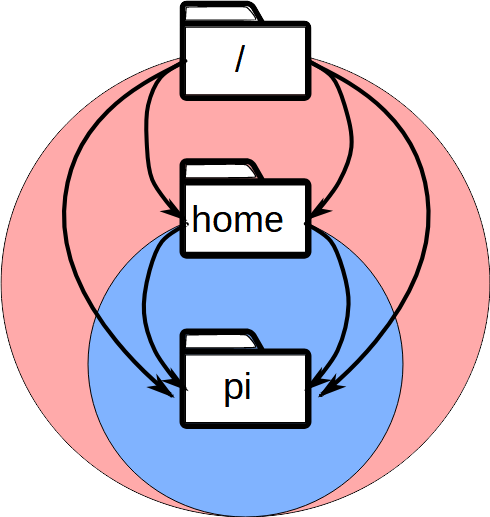
\includegraphics[width=8.068cm,height=9.823cm]{text03-img/text03-img004.png}
\end{figure}
homeは一番上のディレクトリから見ると/home\newline
homeはカレントディレクトリが/のとき./home\newline
homeはカレントディレクトリがhomeのとき./\newline
homeはカレントディレクトリがpiのとき../

piは一番上のディレクトリから見ると/home/pi\newline
piはカレントディレクトリが/のとき./home/pi\newline
piはカレントディレクトリがhomeのとき./pi\newline
piはカレントディレクトリがpiのとき./

\clearpage{\ttfamily
問題3-2}

{\ttfamily\bfseries
このようなディレクトリの関係があります。}



\begin{figure}
\centering
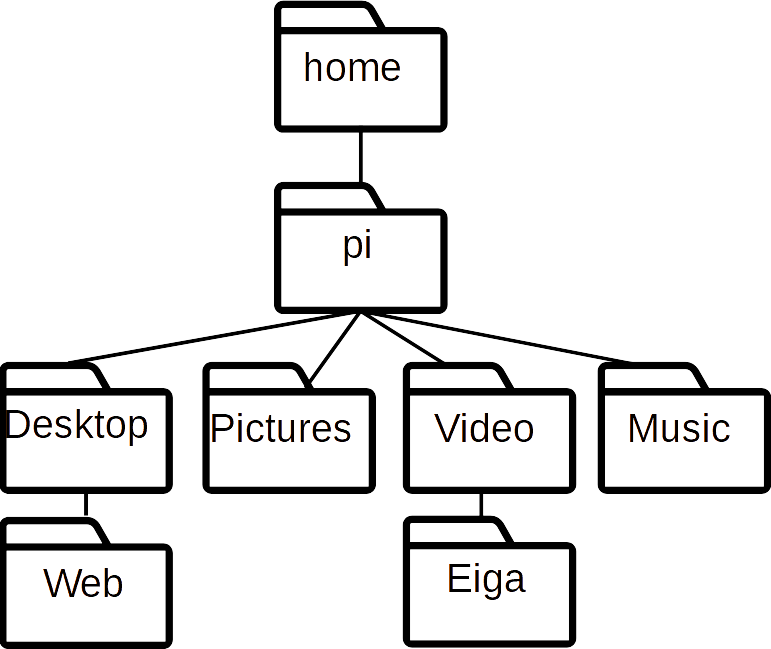
\includegraphics[width=11.742cm,height=8.384cm]{text03-img/text03-img005.png}
\end{figure}
\begin{enumerate}
\item
ホームディレクトリはどれでしょうか
\end{enumerate}

\bigskip


\bigskip

{\ttfamily\bfseries
答え.\_\_\_\_\_\_\_\_\_\_\_\_\_\_\_\_\_\_\_\_\_\_\_\_\_\_\_\_\_\_\_\_\_\_\_\_\_\_\_\_\_\_\_\_\_\_\_\_\_\_\_\_\_\_\_\_\_\_\_\_\_\_\_\_}


\bigskip

\setcounter{saveenum}{\value{enumi}}
\begin{enumerate}
\setcounter{enumi}{\value{saveenum}}
\item
カレントディレクトリが/home/pi/Videoのとき、上のディレクトリはどれでしょうか。
\end{enumerate}

\bigskip


\bigskip

{\ttfamily\bfseries
答え.\_\_\_\_\_\_\_\_\_\_\_\_\_\_\_\_\_\_\_\_\_\_\_\_\_\_\_\_\_\_\_\_\_\_\_\_\_\_\_\_\_\_\_\_\_\_\_\_\_\_\_\_\_\_\_\_\_\_\_\_\_\_\_\_}


\bigskip

\setcounter{saveenum}{\value{enumi}}
\begin{enumerate}
\setcounter{enumi}{\value{saveenum}}
\item
カレントディレクトリが/home/piのとき、下のディレクトリはどれでしょうか。\newline
4つあります。
\end{enumerate}

\bigskip

{\ttfamily\bfseries
答え.\_\_\_\_\_\_\_\_\_\_\_\_\_\_\_\_\_\_\_\_\_\_\_\_\_\_\_\_\_\_\_\_\_\_\_\_\_\_\_\_\_\_\_\_\_\_\_\_\_\_\_\_\_\_\_\_\_\_\_\_\_\_\_\_}


\bigskip

\setcounter{saveenum}{\value{enumi}}
\begin{enumerate}
\setcounter{enumi}{\value{saveenum}}
\item
カレントディレクトリが/home/pi/Desktopのとき、上のディレクトリはどれでしょうか。
\end{enumerate}

\bigskip


\bigskip

{\ttfamily\bfseries
答え.\_\_\_\_\_\_\_\_\_\_\_\_\_\_\_\_\_\_\_\_\_\_\_\_\_\_\_\_\_\_\_\_\_\_\_\_\_\_\_\_\_\_\_\_\_\_\_\_\_\_\_\_\_\_\_\_\_\_\_\_\_\_\_\_}


\bigskip

\setcounter{saveenum}{\value{enumi}}
\begin{enumerate}
\setcounter{enumi}{\value{saveenum}}
\item
カレントディレクトリが/home/pi/Desktopのとき、下のディレクトリはどれでしょうか。
\end{enumerate}

\bigskip


\bigskip

{\ttfamily\bfseries
答え.\_\_\_\_\_\_\_\_\_\_\_\_\_\_\_\_\_\_\_\_\_\_\_\_\_\_\_\_\_\_\_\_\_\_\_\_\_\_\_\_\_\_\_\_\_\_\_\_\_\_\_\_\_\_\_\_\_\_\_\_\_\_\_\_}

\clearpage\section{ターミナルでファイルとディレクトリを使ってみよう}
[Warning: Draw object ignored]

\begin{figure}
\centering
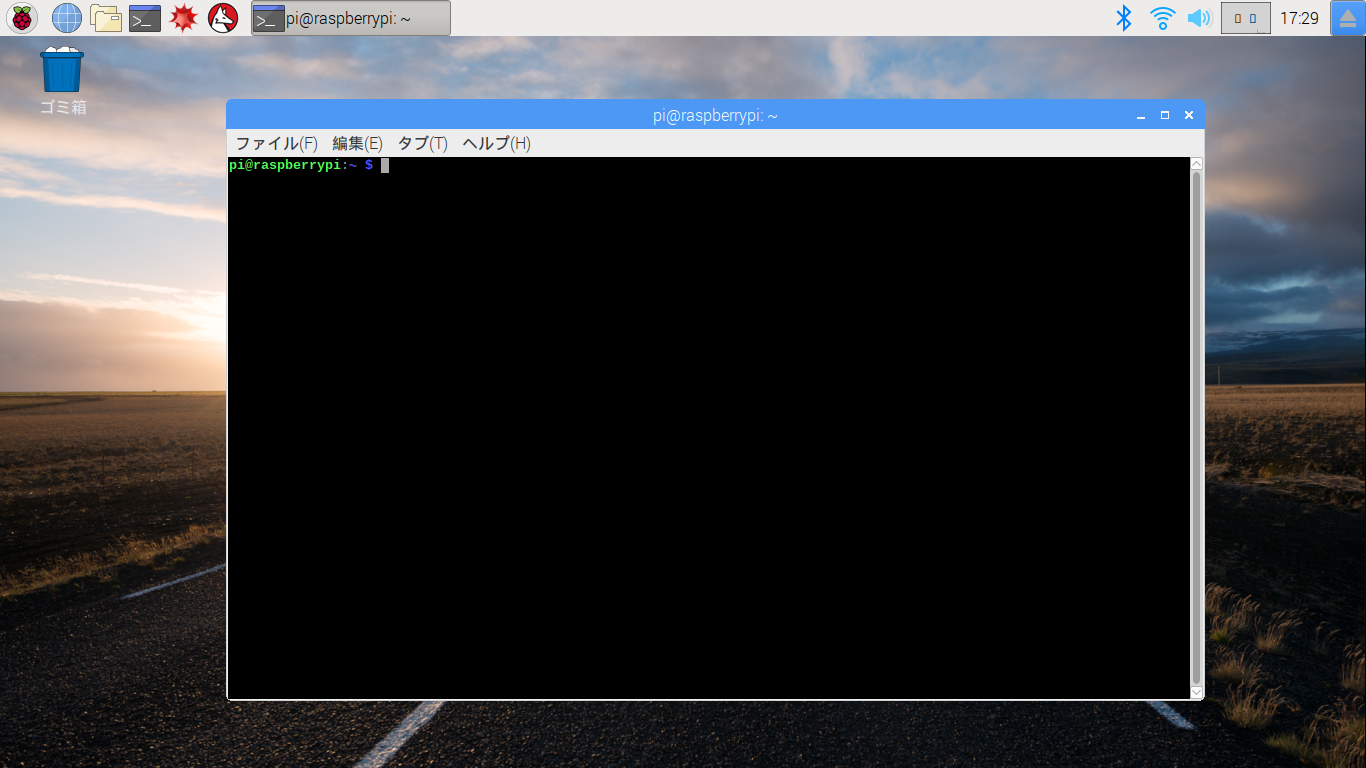
\includegraphics[width=17.006cm,height=9.56cm]{text03-img/text03-img006.png}
\end{figure}
\subsection{コマンドについて知ろう}
ターミナルでは\textbf{コマンド}を使ってコンピュータとやりとりをします。コマンドとはコンピュータにあたえる\textbf{命令}のことです。コマンドは下のようなかたちで書きます。\textbf{Enterキー(エンターキー)を押して}送ります。EnterキーはReturn(リターン)キーと呼ぶこともあります。

コマンド\textcolor[rgb]{1.0,0.2,0.2}{
}オプション\textcolor[rgb]{1.0,0.2,0.2}{ }引数ひきすう1
引数ひきすう2

コマンドは動作、引数はそうさのたいしょうです。使うときは次のことに気を付けましょう。

\begin{itemize}
\item 半角英数字でかくこと
\item 間にスペース(空白)をいれること
\end{itemize}

\bigskip

今回はわかりやすいように、スペースが赤くなっています。次回からは赤くないのでしっかり覚えましょう。

\subsection{}
\clearpage\subsection{コマンドを使ってみよう}
\subsubsection{自分がどのディレクトリにいるかしろう}
\textbf{pwd}\newline
カレントディレクトリ(自分が今いるディレクトリ)が出てきます。\newline
{\textless}例{\textgreater}pwdと入力してみます。

\subsubsection*{}
\begin{figure}
\centering
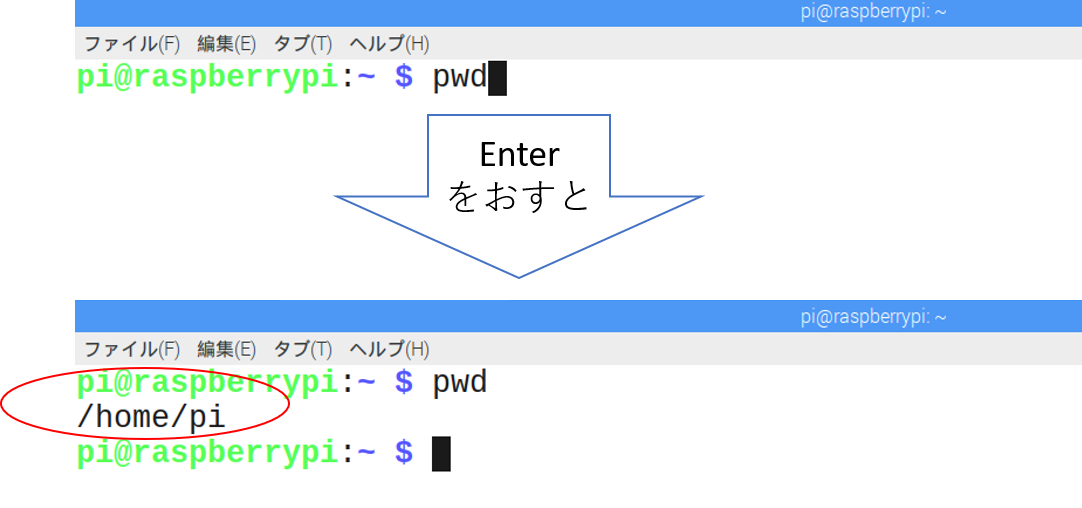
\includegraphics[width=15.42cm,height=7.239cm]{text03-img/text03-img007.png}
\end{figure}
{\ttfamily
問題3-3}

\begin{enumerate}
\item
実際にpwdを使って、カレントディレクトリが出ることを確かめましょう。\newline
出てきたカレントディレクトリを書いてください。
\end{enumerate}

\bigskip

{\ttfamily\bfseries
答え.\_\_\_\_\_\_\_\_\_\_\_\_\_\_\_\_\_\_\_\_\_\_\_\_\_\_\_\_\_\_\_\_\_\_\_\_\_\_\_\_\_\_\_\_\_\_\_\_\_\_\_\_\_\_\_\_\_\_\_\_\_\_\_\_\_\_\_\_\_\_}

\subsubsection{}
\clearpage\subsubsection{ディレクトリの中を見てみよう}
\textbf{ls {}-F ディレクトリ}\newline
ディレクトリの中のファイルやディレクトリが出てきます。ファイルはピンクの文字、ディレクトリは青い文字になっています。\newline
{\textless}例{\textgreater}ls
{}-Fだけだとカレントディレクトリの中を見ることができます。\newline
{\textless}例{\textgreater}画像というディレクトリの中を見る場合は
ls {}-F 画像/と打ちます。\newline
ディレクトリの中にあるファイルは人によってちがいます。\newline


\begin{figure}
\centering
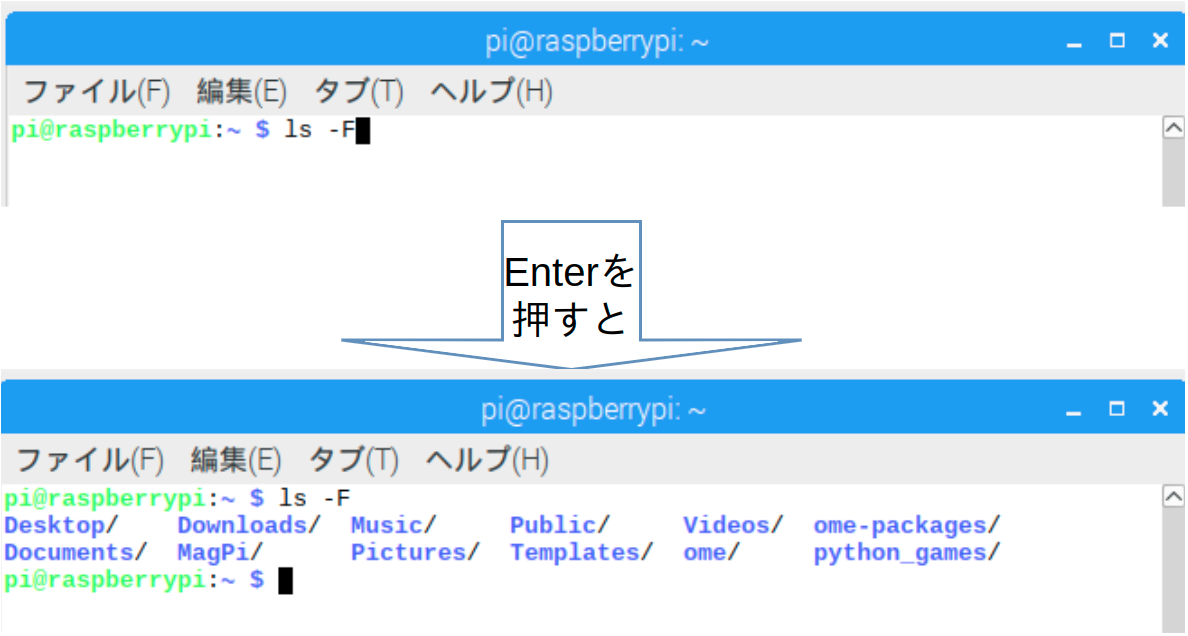
\includegraphics[width=17.006cm,height=6.14cm]{text03-img/text03-img008.png}
\end{figure}
\begin{figure}
\centering
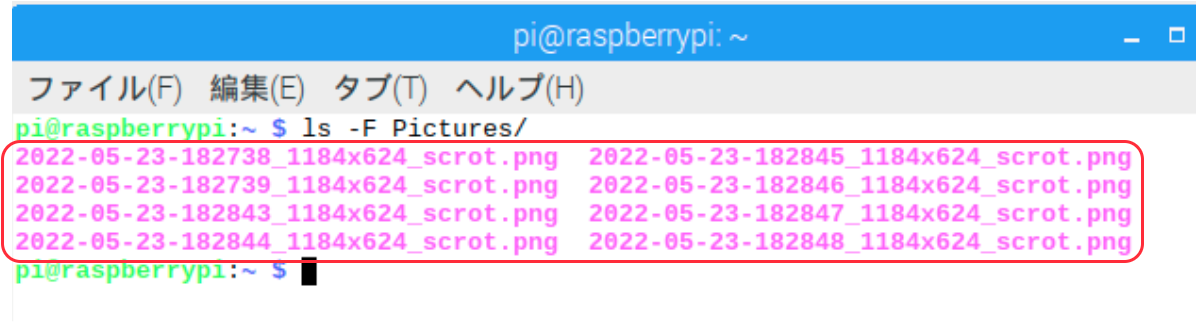
\includegraphics[width=15.122cm,height=2.607cm]{text03-img/text03-img009.png}
\end{figure}
{\ttfamily
問題3-4}

ls
{}-Fと入力して出てきたファイルとディレクトリの名前を1つずつ書きましょう。

\subsubsection{}
\subsubsection{}
\subsubsection[\ \ 答え.\_\_\_\_\_\_\_\_\_\_\_\_\_\_\_\_\_\_\_\_\_\_\_\_\_\_\_\_\_\_\_\_\_\_\_\_\_\_\_\_\_\_\_\_\_\_\_\_\_\_\_\_\_\_\_\_\_\_\_\_\_\_\_\_]{\ \ 答え.\_\_\_\_\_\_\_\_\_\_\_\_\_\_\_\_\_\_\_\_\_\_\_\_\_\_\_\_\_\_\_\_\_\_\_\_\_\_\_\_\_\_\_\_\_\_\_\_\_\_\_\_\_\_\_\_\_\_\_\_\_\_\_\_}
\subsubsection{}
ls {}-F 画像
/と入力して出てきたファイルかディレクトリの名前を1つ書きましょう。

\subsubsection{}
\subsubsection{}
\subsubsection{答え.\_\_\_\_\_\_\_\_\_\_\_\_\_\_\_\_\_\_\_\_\_\_\_\_\_\_\_\_\_\_\_\_\_\_\_\_\_\_\_\_\_\_\_\_\_\_\_\_\_\_\_\_\_\_\_\_\_\_\_\_\_\_\_\_}
\clearpage\subsubsection{ディレクトリへ移動してみよう}
\textbf{cd ディレクトリ}\newline
指定したディレクトリへ移動することができます。

{\textless}例{\textgreater}画像ディレクトリに移動するときはcd
画像/と入力します。\newline
赤まるで囲まれた部分が変わっています。ここはカレントディレクトリが書かれています。\newline
\textbf{cd}\newline
ホームディレクトリに移動できます。\newline
{\textless}例{\textgreater}画像ディレクトリに移動したあとに、cdとだけ入力するとホームディレクトリに移動できます。ディレクトリを入力しなくてもホームディレクトリに移動できました。

\begin{figure}
\centering
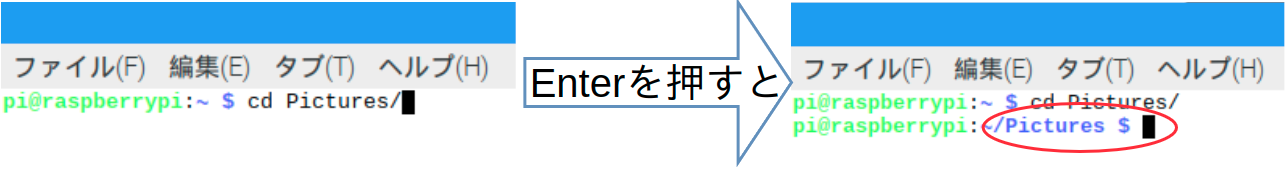
\includegraphics[width=17.006cm,height=2.339cm]{text03-img/text03-img010.png}
\end{figure}
\begin{figure}
\centering
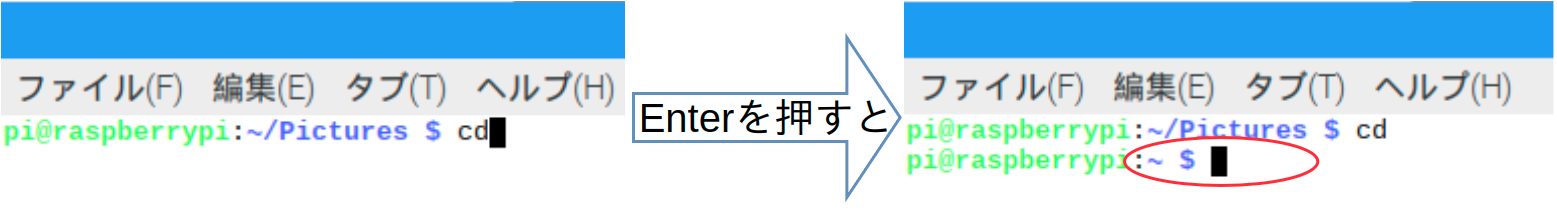
\includegraphics[width=16.715cm,height=2.286cm]{text03-img/text03-img011.png}
\end{figure}
{\ttfamily
問題3-5}

\begin{enumerate}
\item cd 画像/と入力して画像
ディレクトリに移動してみましょう。\newline
${\square}$ $\leftarrow $
移動できたらチェックしましょう。
\item
cdと入力してホームディレクトリに移動してみましょう。\newline
${\square}$ $\leftarrow $
移動できたらチェックしましょう。
\end{enumerate}
\subsubsection{}
\clearpage\subsubsection{便利なTab(タブ)キーを使ってみよう}
入力したい文字の途中まで入力してから、Tabキーを押すと、コンピュータが残りの文字を推測してくれます。似たような文字があるときは、候補を出してくれます。\newline
\newline
{\textless}例{\textgreater}コマンドを入力する途中でTabキーを使ってみます。\newline
\ \ どれかわからないので、コマンドの候補を出してくれました。

%\newline
{\textless}例{\textgreater}ファイルやディレクトリの名前の途中でTabキーを使ってみます。\newline
\ \ コンピュータが残りの文字を入力してくれました。

\begin{figure}
\centering
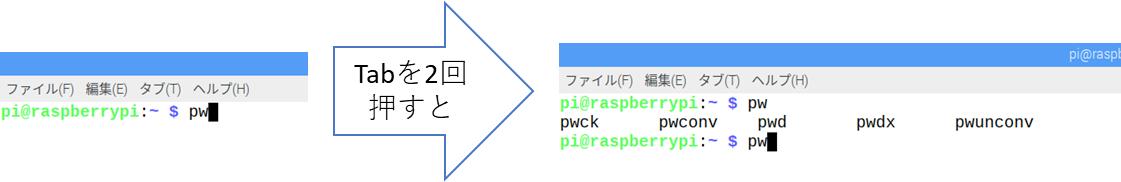
\includegraphics[width=17.006cm,height=2.76cm]{text03-img/text03-img012.png}
\end{figure}
%\newline
{\textless}例{\textgreater}ファイルやディレクトリの名前の途中でTabキーを使ってみます。\newline
\ \ どれかわからないので、ディレクトリやファイルの候補を出してくれました。

\begin{figure}
\centering
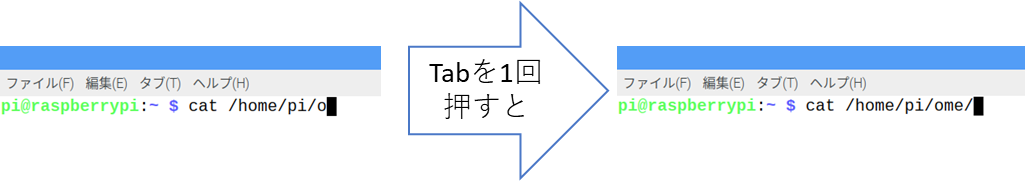
\includegraphics[width=17.006cm,height=3.002cm]{text03-img/text03-img013.png}
\end{figure}
\subsubsection[]{}
\begin{figure}
\centering
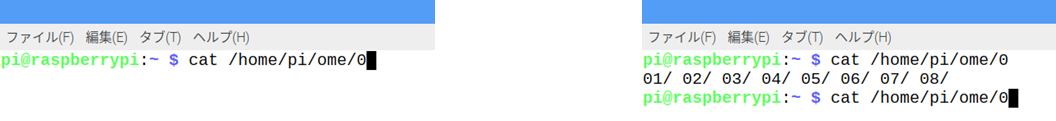
\includegraphics[width=17.006cm,height=1.949cm]{text03-img/text03-img014.png}
\end{figure}
\subsubsection{}
\subsubsection{}
\clearpage\subsubsection{ファイルの中身を見てみよう}
\textbf{cat ファイル}\newline
ファイルに書かれている文字を表示することができます。\newline
{\textless}例{\textgreater}syousetu.txtに書かれている文字を表示します。



\begin{figure}
\centering
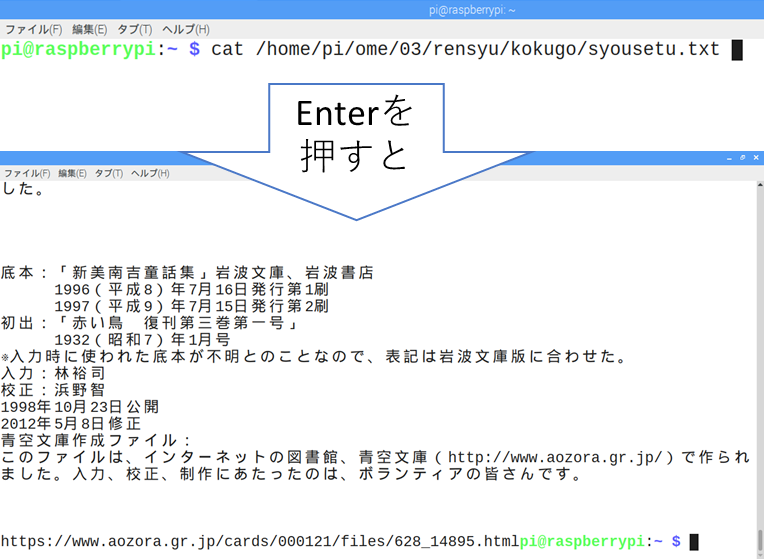
\includegraphics[width=12.938cm,height=9.467cm]{text03-img/text03-img015.png}
\end{figure}
{\ttfamily
問題3-6}

\begin{enumerate}
\item cat
/home/pi/ome/03/rensyu/kokugo/syousetu.txtと入力してみましょう。\newline
表示された小説の題名はなんでしょうか。\newline

\end{enumerate}

\bigskip

{\ttfamily\bfseries
答え\_\_\_\_\_\_\_\_\_\_\_\_\_\_\_\_\_\_\_\_\_\_\_\_\_\_\_\_\_\_\_\_\_\_\_\_\_\_\_\_\_\_\_\_\_\_\_\_\_\_\_\_\_\_\_\_\_\_\_\_\_\_\_\_\_\_\_\_\_\_\_}

\subsubsection{}
\clearpage\subsubsection{コピーしてみよう}
\textbf{cp ファイル1 ファイル2}\newline
ファイルをコピーすることができます。\newline
{\textless}例{\textgreater}ome/03/rensyu/rika/rika.pngをホームディレクトリに、rika2.pngという名前でコピーします。ls
{}-Fするとrika2.pngがコピーされていることがわかります。



\begin{figure}
\centering
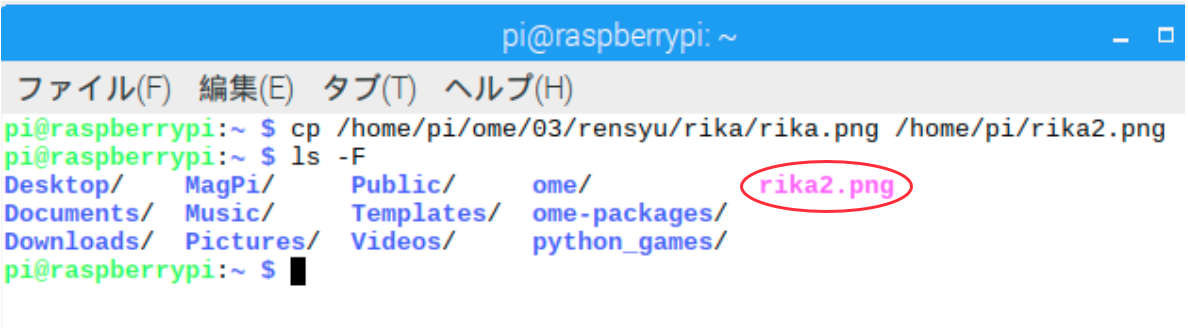
\includegraphics[width=17.133cm,height=3.304cm]{text03-img/text03-img016.png}
\end{figure}
\textbf{cp {}-r ディレクトリ1
ディレクトリ2}\newline
ディレクトリをコピーすることができます\newline
{\textless}例{\textgreater}ome/03/rensyu/rikaをホームディレクトリに、rikaという名前でコピーします。ls
{}-Fするとrikaディレクトリがコピーされていることがわかります。\newline


\begin{figure}
\centering
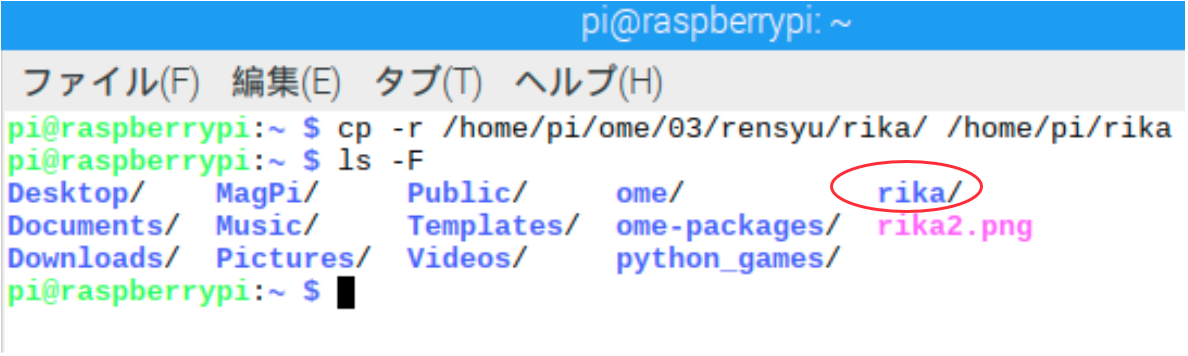
\includegraphics[width=17.618cm,height=3.81cm]{text03-img/text03-img017.png}
\end{figure}
{\ttfamily
問題3-7}

\begin{enumerate}
\item cp /home/pi/ome/03/rensyu/rika/rika.png
/home/pi/rika2.pngと入力してみましょう。ls
{}-Fと打ってrika2.pngがコピーされているか見てみましょう。\newline
${\square}$ $\leftarrow $
コピーできたらチェックしましょう。
\item cp {}-r /home/pi/ome/03/rensyu/rika
/home/pi/rikaと入力してみましょう。\newline
ls
{}-Fと打ってrikaディレクトリがコピーされているか見てみましょう。\newline
${\square}$ $\leftarrow $
コピーできたらチェックしましょう。
\end{enumerate}
\subsubsection{}
\clearpage\subsubsection{ファイルやディレクトリを移動してみよう}
\textbf{mv ファイルやディレクトリ 移動先}\newline
ファイルやディレクトリを移動することができます。\newline
{\textless}例{\textgreater}rika2.pngをrikaディレクトリに移動します。ls
{}-F
rikaするとrika2.pngがrikaディレクトリの中に移動されていることがわかります。

{\ttfamily
問題3-8}

\begin{figure}
\centering
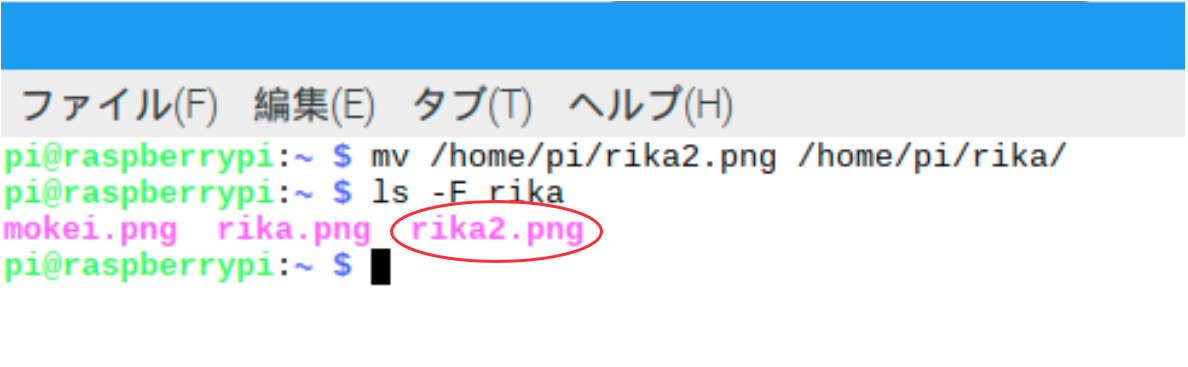
\includegraphics[width=11.719cm,height=4.17cm]{text03-img/text03-img018.png}
\end{figure}
\begin{enumerate}
\item mv rika2.png rika/と入力してみましょう。\newline
ls {}-F
rikaと打ってrika2.pngがrikaディレクトリの下に移動しているか見てみましょう。\newline
${\square}$ $\leftarrow $
コピーできたらチェックしましょう。\newline

\end{enumerate}
\subsubsection{名前を変えてみよう}
\textbf{mv 名前 変えた後の名前}\newline
ファイルやディレクトリの名前を変えることができます。\newline
{\textless}例{\textgreater}rika2.pngをbika.pngに名前を変えます。ls
{}-F
rikaで、名前が変わっているとわかります。

\begin{figure}
\centering
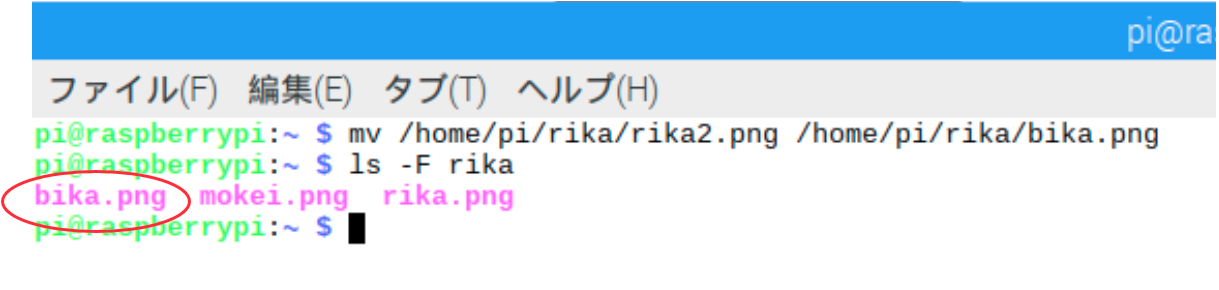
\includegraphics[width=13.279cm,height=2.882cm]{text03-img/text03-img019.png}
\end{figure}
{\ttfamily
問題3-9}

\begin{enumerate}
\item mv rika/rika2.png
rika/bika.pngと入力してみましょう。\newline
ls {}-F
rikaと打ってrika2.pngがbika.pngに変わっているか見てみましょう。\newline
${\square}$ $\leftarrow $
bika.pngがあったらチェックしましょう。
\end{enumerate}
\subsubsection{}
\clearpage\subsubsection{テキストファイルを作ってみよう}
\textbf{leafpad ファイル}\newline
leafpadを使ってファイルを作ることができます。\newline
{\textless}例{\textgreater}my.txtを作り、文字を書いて保存します。

{\ttfamily
問題3-10}

\begin{figure}
\centering
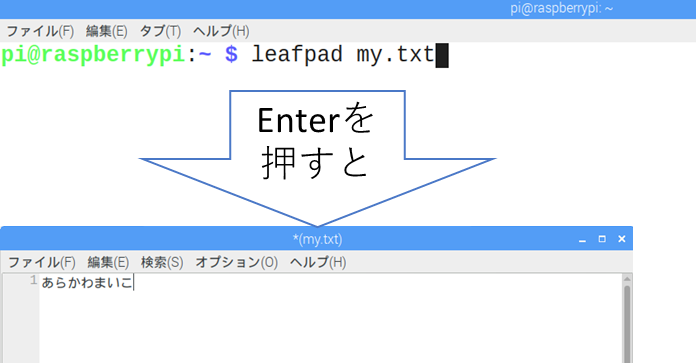
\includegraphics[width=10.539cm,height=5.498cm]{text03-img/text03-img020.png}
\end{figure}
\begin{enumerate}
\item leafpad
my.txtと入力してみましょう。リーフパッドが開きました。\newline
自分の名前を書いて保存しましょう。ls
{}-Fと入力してmy.txtがあるか見てみましょう。\newline
${\square}$ $\leftarrow $
my.txtがあったらチェックしましょう。\newline

\end{enumerate}
\subsubsection{ディレクトリを作ってみよう}
\textbf{mkdir ディレクトリ}\newline
ディレクトリを作ることができます。\newline
{\textless}例{\textgreater}myディレクトリを作ります。

{\ttfamily
問題3-11}

\begin{figure}
\centering
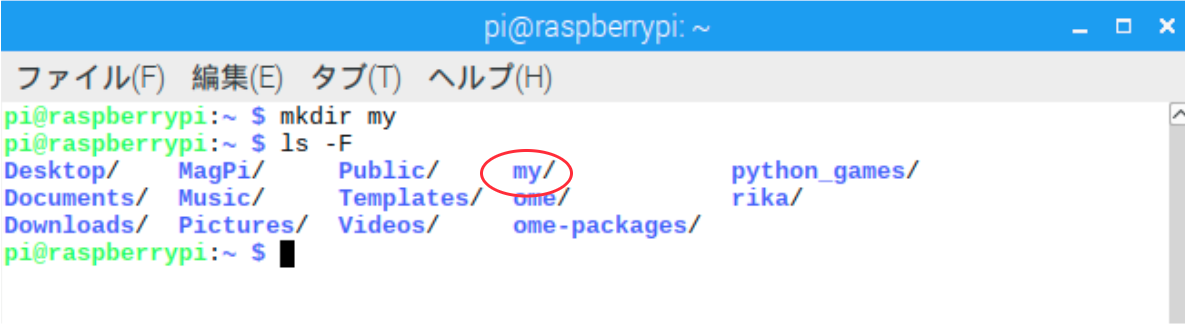
\includegraphics[width=15.794cm,height=3.078cm]{text03-img/text03-img021.png}
\end{figure}
\begin{enumerate}
\item mkdir myと入力してみましょう。\newline
ls
{}-Fと打ってmyディレクトリができているか見てみましょう。\newline
${\square}$ $\leftarrow $
myディレクトリがあったらチェックしましょう。\newline

\end{enumerate}
\subsubsection{消してみよう}
ファイルやディレクトリは一度消すと\textbf{元には戻りません}。気を付けましょう。

\textbf{rm ファイル}\newline
ファイルを消すことができます。\newline
{\textless}例{\textgreater}my.txtを消します。



\begin{figure}
\centering
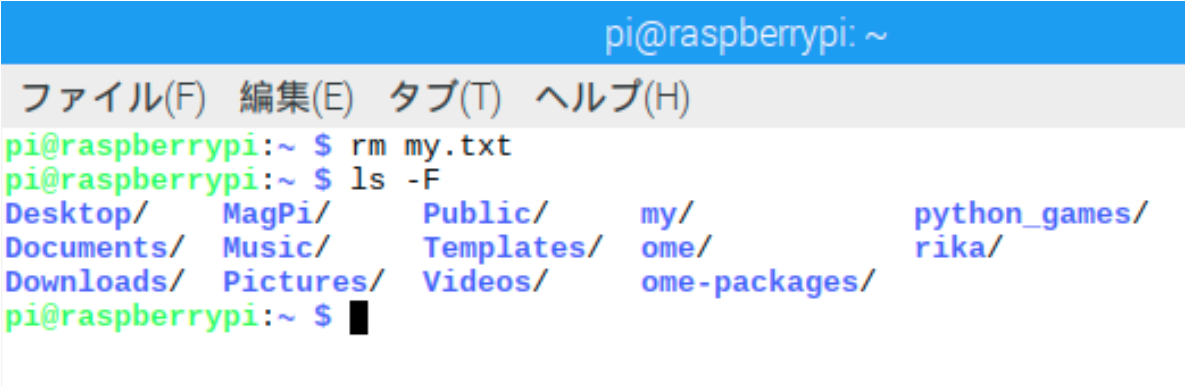
\includegraphics[width=13.49cm,height=3.293cm]{text03-img/text03-img022.png}
\end{figure}
\textbf{rm {}-r ディレクトリ}\newline
ディレクトリを消すことができます。\newline
{\textless}例{\textgreater}myディレクトリを消します。\newline


\begin{figure}
\centering
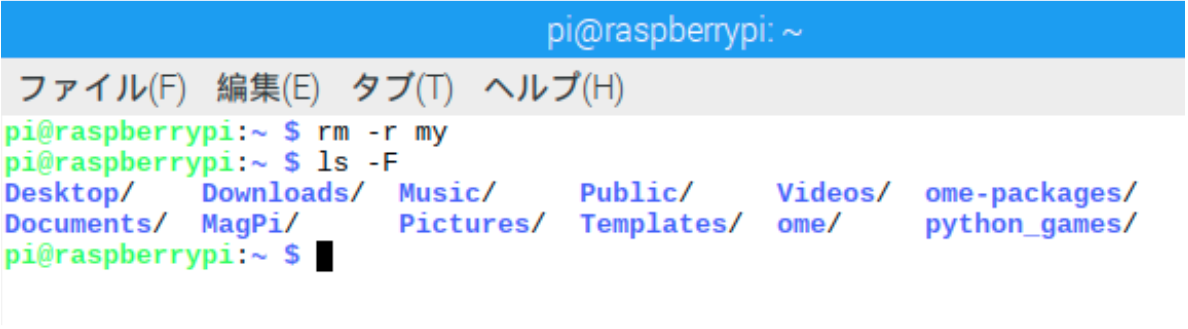
\includegraphics[width=19.006cm,height=2.36cm]{text03-img/text03-img023.png}
\end{figure}
{\ttfamily
問題3-12}

\begin{enumerate}
\item rm my.txtと入力してみましょう。\newline
ls
{}-Fと打ってmy.txtが消えているか見てみましょう。\newline
${\square}$ $\leftarrow $
消えていたらチェックしましょう。
\item rm {}-r myと入力してみましょう。\newline
ls -F
と打ってmyディレクトリが消えているか見てみましょう。\newline
${\square}$ $\leftarrow $
消えていたらチェックしましょう。
\end{enumerate}
\clearpage\subsubsection{ファイルの中身を見てみよう(2)}
\textbf{less ファイルの名前}\newline
ファイルに書かれている文字を一画面ずつ見ることができます。\newline
{\textless}例{\textgreater}syousetu.txtの中を見てみます。

eを押すと一行進みます。\newline
yを押すと一行戻ります。\newline
qを押すと終わります。

\begin{figure}
\centering
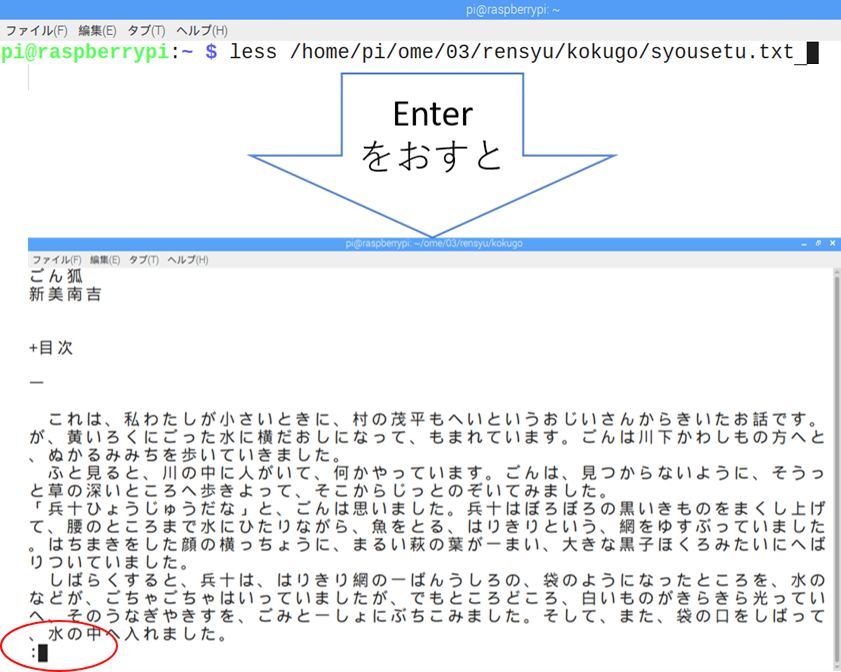
\includegraphics[width=14.242cm,height=11.381cm]{text03-img/text03-img024.png}
\end{figure}
{\ttfamily
問題3-13}

\begin{enumerate}
\item less\textcolor[rgb]{1.0,0.2,0.2}{
}/home/pi/ome/03/rensyu/kokugo/syousetu.txtと入力してみましょう。\newline
${\square}$ $\leftarrow $
小説が表示されたらチェックしましょう。
\item qを押して終わってみましょう。\newline
${\square}$ $\leftarrow $
小説が消えたらチェックしましょう。
\end{enumerate}
\subsubsection*{}
\subsubsection{}
\clearpage\subsubsection{応用:GIFアニメーションの作成}
gifアニメーションを使ってスライドショー作ってみましょう。gifとは画像ファイルのフォーマットの1つで、アニメーションを表現することもできます。

\begin{enumerate}
\item \begin{enumerate}
\item ディレクトリ slideshow
を/home/piに作りましょう。
\item
スライドショーの素材(パラパラ漫画の一枚一枚)を集めます。インターネットで画像を検索したり、Gimpで作ったりしましょう。画像は今作ったslideshowというディレクトリに保存しましょう。
\item
画像の名前が連番になるように名前を変更します。00.jpg
01.jpg 02.jpg {\dots}
のようにスライドショーで表示したい順番の番号を名前にしましょう。
\item Gimpを開きます。「ファイル」$\rightarrow
「開く$/インポート」で「画像ファイルを開く」ウィンドウを出し、最初の一枚目を選択して開きます。Gimpで「ファイル」$\rightarrow
「レイヤーとして開く」で、$2番め以降の全てのファイルを選択して開きましょう。Shiftキーを押しながらクリックすることで複数選択できます。選択するときは、「名前」をクリックして名前の順に並び替えておきましょう。
\begin{figure}
\centering
\caption[: ]{ 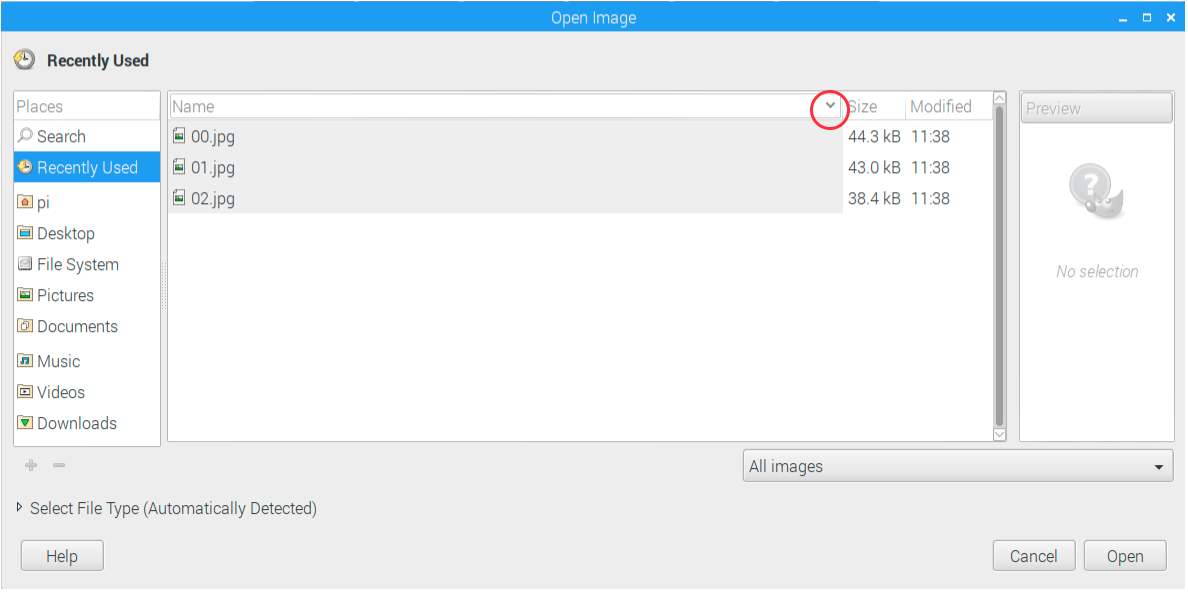
\includegraphics[width=14.88cm,height=11.158cm]{text03-img/text03-img025.png} \newline
: }

\end{figure}
\item Gimpで「ファイル」$\rightarrow
「名前をつけてエクスポート」をクリックします。名前を$slideshow.gifとし、エクスポートボタンを押します。
\item 「画像をエクスポート:
GIF形式」というウィンドウが出るので、「アニメーションとしてエクスポート」にチェック、「指定しない場合のディレイ」をお好みに(2000ミリ秒くらいがオススメ)、「指定しない場合のフレーム処理」を「レイヤーごとに1フレーム(置換)」に、「全フレームのディレイにこの値を使用」にチェック、「全フレームのフレーム処理にこの値を使用」にチェックをしてエクスポートボタンを押します。
\begin{figure}
\centering
\caption[: ]{ 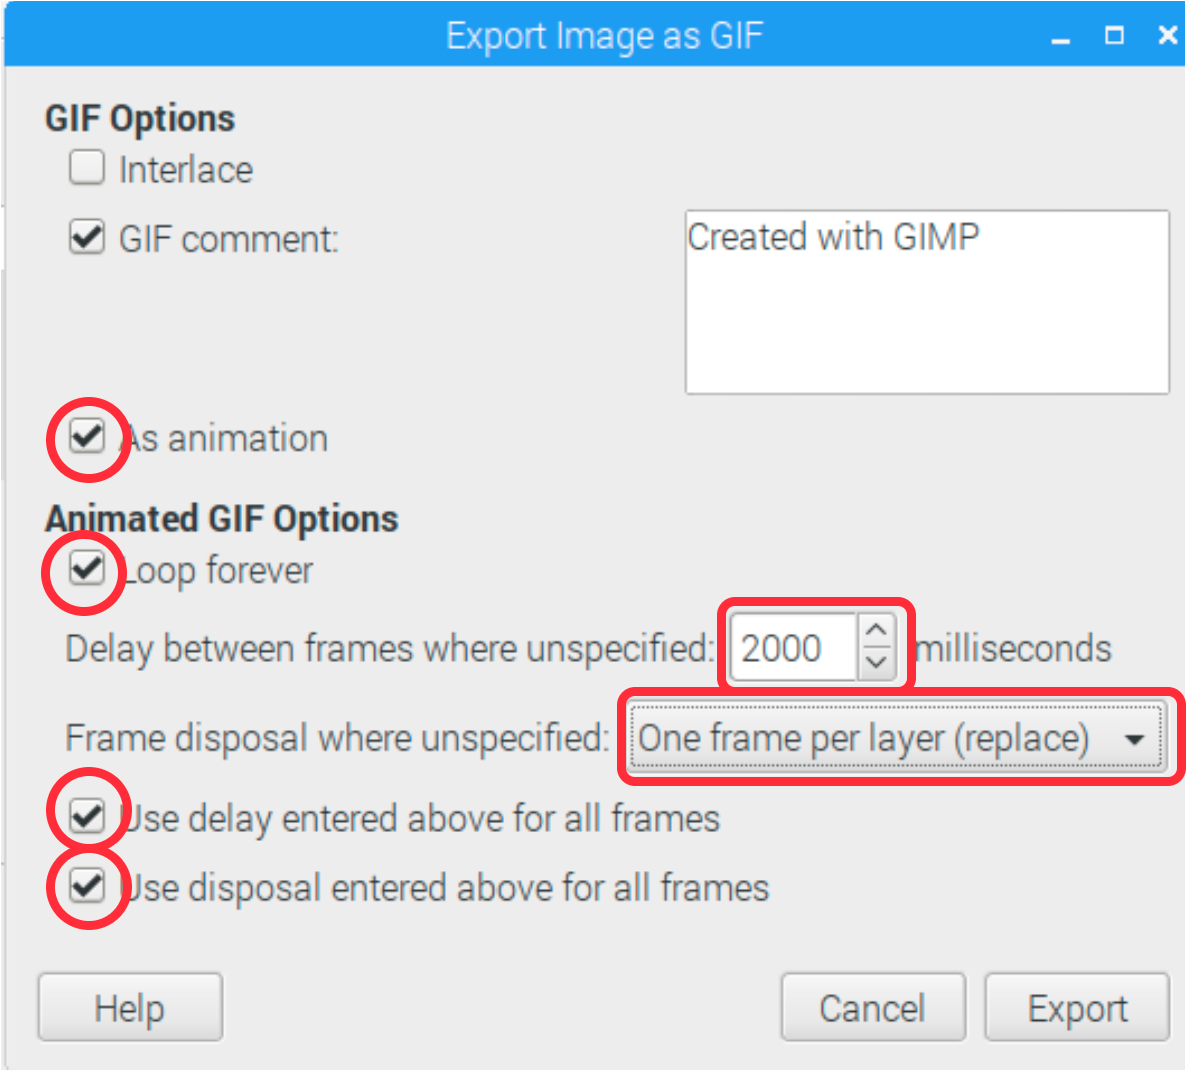
\includegraphics[width=14.265cm,height=11.434cm]{text03-img/text03-img026.png} \newline
: }

\end{figure}
\item
出来上がった画像をみてみましょう。下記どちらかのコマンドでみることができます。\newline
chromium-browser slideshow.gif\newline
gpicview slideshow.gif
\end{enumerate}
\end{enumerate}
{\ttfamily
問題3-14}

\begin{enumerate}
\item
2.2.13にしたがって、オリジナルのGIFアニメーションを作成しましょう。\newline
${\square}$ $\leftarrow $
できたらチェックしましょう。
\end{enumerate}
\subsubsection{おまけ:こんなメッセージが出たときは}
コマンドが違います。スペル(アルファベット)があっているか見てみましょう。



\begin{figure}
\centering
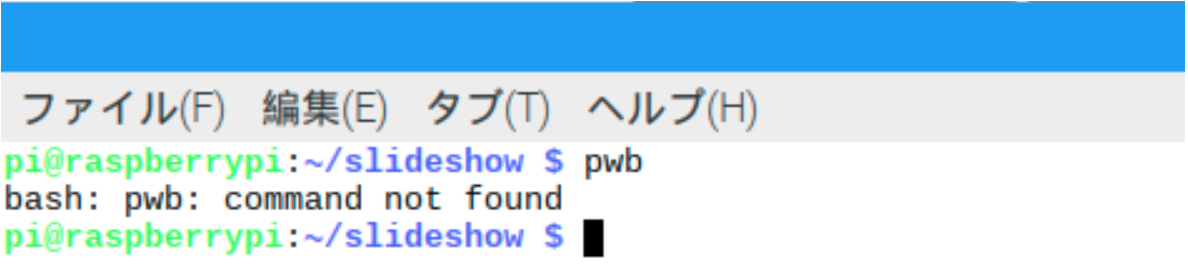
\includegraphics[width=15.136cm,height=3.069cm]{text03-img/text03-img027.png}
\end{figure}
ディレクトリやディレクトリの名前が違います。スペルがあっているか見てみましょう。



\begin{figure}
\centering
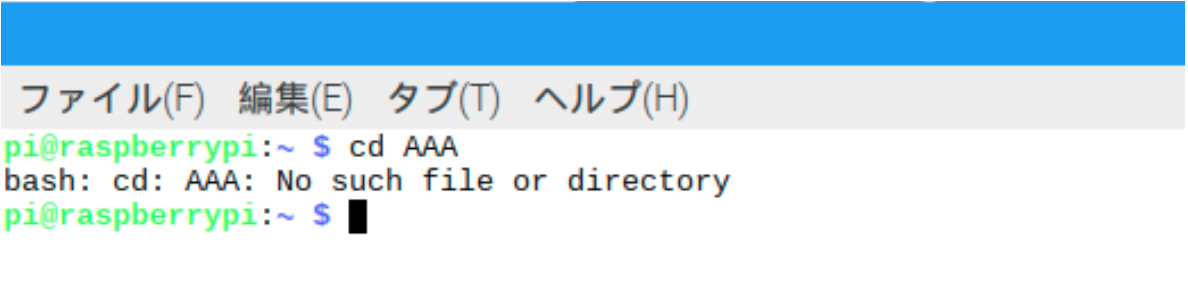
\includegraphics[width=17.006cm,height=2.635cm]{text03-img/text03-img028.png}
\end{figure}
\subsubsection{豆知識}
コマンドは英文や英単語の省略になっています。

pwd: print working directory $\rightarrow $
ワーキングディレクトリを表示する\newline
cd: change directory $\rightarrow $ ディレクトリを変える\newline
cat: concatenate $\rightarrow $ 結合する\newline
mv: move $\rightarrow $ 移動する\newline
mkdir: make directory $\rightarrow $ ディレクトリを作る\newline
rm: remove $\rightarrow $ 消す


\bigskip

\subsubsection{rensyuディレクトリを最初の状態に戻すには}
/home/pi/ome/03/rensyuディレクトリはファイルそうさの練習用のディレクトリです。練習することで、内容が変わってしまいます。授業が始まる前の状態に戻すには次のコマンドを使います。rensyuディレククトリの下の自分で作ったファイルやディレクトリは消えるので注意してください。

\begin{enumerate}
\item cd\textcolor[rgb]{1.0,0.2,0.2}{ }/home/pi/ome/03/
\item tar\textcolor[rgb]{1.0,0.2,0.2}{ }{}-{}-recursive-unlink {}-zxvf rensyu.tar.gz
\end{enumerate}
\clearpage{\ttfamily
まとめ問題3-15}

ターミナルを開いて、コマンドを使って問題をといてみましょう。

\begin{figure}
\centering
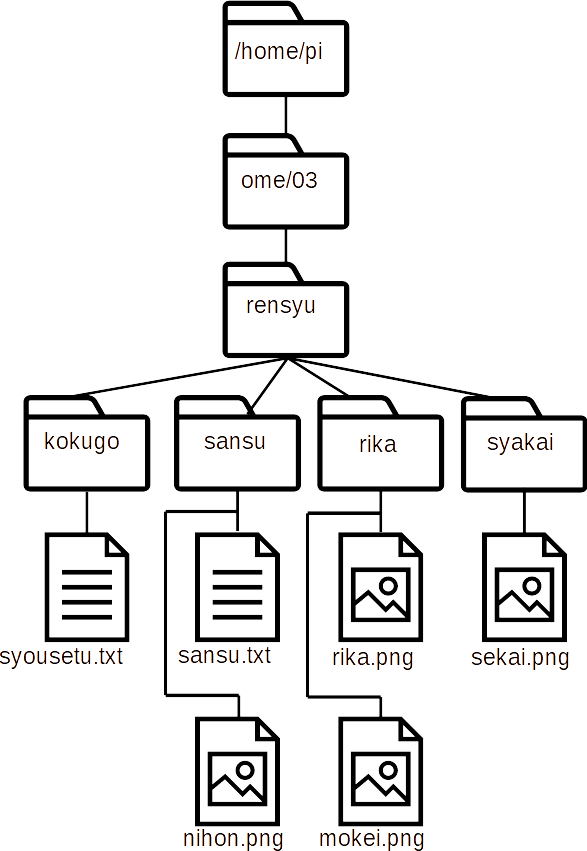
\includegraphics[width=9.585cm,height=14.088cm]{text03-img/text03-img029.png}
\end{figure}
\begin{enumerate}
\item
カレントディレクトリはどこか調べてみましょう。
\end{enumerate}

\bigskip


\bigskip

\setcounter{saveenum}{\value{enumi}}
\begin{enumerate}
\setcounter{enumi}{\value{saveenum}}
\item \setcounter{saveenum}{\value{enumii}}
\begin{enumerate}
\setcounter{enumii}{\value{saveenum}}
\item \setcounter{saveenum}{\value{enumiii}}
\begin{enumerate}
\setcounter{enumiii}{\value{saveenum}}
\item[] {\ttfamily\bfseries
答え.\_\_\_\_\_\_\_\_\_\_\_\_\_\_\_\_\_\_\_\_\_\_\_\_\_\_\_\_\_\_\_\_\_\_\_\_\_\_\_\_\_\_\_\_\_\_\_\_\_\_\_\_\_\_\_\_\_\_\_\_\_\_\_\_}
\end{enumerate}
\end{enumerate}

\bigskip
\item
カレントディレクトリの中身を見てみましょう。


\bigskip
\end{enumerate}

\bigskip

{\ttfamily\bfseries
答え.\_\_\_\_\_\_\_\_\_\_\_\_\_\_\_\_\_\_\_\_\_\_\_\_\_\_\_\_\_\_\_\_\_\_\_\_\_\_\_\_\_\_\_\_\_\_\_\_\_\_\_\_\_\_\_\_\_\_\_\_\_\_\_\_}


\bigskip

\setcounter{saveenum}{\value{enumi}}
\begin{enumerate}
\setcounter{enumi}{\value{saveenum}}
\item /home/pi/ome/03/rensyuに移動してみましょう。\newline
${\square}$ $\leftarrow $
できたらチェックしましょう。
\end{enumerate}

\bigskip

\setcounter{saveenum}{\value{enumi}}
\begin{enumerate}
\setcounter{enumi}{\value{saveenum}}
\item \clearpage
rensyuディレクトリの中身を調べてみましょう。どんなディレクトリがありますか?
\end{enumerate}

\bigskip

\setcounter{saveenum}{\value{enumi}}
\begin{enumerate}
\setcounter{enumi}{\value{saveenum}}
\item[] 
\bigskip

\setcounter{saveenum}{\value{enumii}}
\begin{enumerate}
\setcounter{enumii}{\value{saveenum}}
\item \setcounter{saveenum}{\value{enumiii}}
\begin{enumerate}
\setcounter{enumiii}{\value{saveenum}}
\item[] {\ttfamily\bfseries
答え.\_\_\_\_\_\_\_\_\_\_\_\_\_\_\_\_\_\_\_\_\_\_\_\_\_\_\_\_\_\_\_\_\_\_\_\_\_\_\_\_\_\_\_\_\_\_\_\_\_\_\_\_\_\_\_\_\_\_\_\_\_\_\_\_}
\end{enumerate}

\bigskip
\end{enumerate}
\item
一番上からのディレクトリからsyousetu.txtファイルの中身を見てみましょう。\newline
${\square}$ $\leftarrow $
できたらチェックしましょう。
\item
カレントディレクトリからsyousetu.txtファイルの中身を見てみましょう。\newline
${\square}$ $\leftarrow $
できたらチェックしましょう。
\item
kokugoディレクトリに移動してから、syousetu.txtファイルの中身を見てみましょう。\newline
${\square}$ $\leftarrow $
できたらチェックしましょう。
\item 内容はぜんぶ同じでしたか?
\end{enumerate}

\bigskip

\setcounter{saveenum}{\value{enumi}}
\begin{enumerate}
\setcounter{enumi}{\value{saveenum}}
\item[] 
\bigskip

\setcounter{saveenum}{\value{enumii}}
\begin{enumerate}
\setcounter{enumii}{\value{saveenum}}
\item \setcounter{saveenum}{\value{enumiii}}
\begin{enumerate}
\setcounter{enumiii}{\value{saveenum}}
\item[] {\ttfamily\bfseries
答え.\_\_\_\_\_\_\_\_\_\_\_\_\_\_\_\_\_\_\_\_\_\_\_\_\_\_\_\_\_\_\_\_\_\_\_\_\_\_\_\_\_\_\_\_\_\_\_\_\_\_\_\_\_\_\_\_\_\_\_\_\_\_\_\_}
\end{enumerate}
\end{enumerate}

\bigskip
\item
rikaディレクトリの下にあるmokei.pngをコピーして\newline
rikaディレクトリの中にmokei2.pngを作りましょう。\newline
${\square}$ $\leftarrow $
できたらチェックしましょう。
\item rikaディレクトリをコピーして、\newline
rensyuディレクトリの下にrika2ディレクトリを作りましょう。\newline
${\square}$ $\leftarrow $
できたらチェックしましょう。
\item
rensyuディレクトリの下にあるkanji.txtをkokugoディレクトリの下に移動しましょう。\newline
${\square}$ $\leftarrow $
できたらチェックしましょう。
\item
sansuディレクトリの下にあるnihon.pngをsyakaiディレクトリの下に移動しましょう。\newline
${\square}$ $\leftarrow $
できたらチェックしましょう。
\item
rekisiディレクトリを作り、syakaiディレクトリの下に移動しましょう。\newline
${\square}$ $\leftarrow $
できたらチェックしましょう。
\item
rensyuディレクトリの下にあるoda.jpgをsyakai/rekisiディレクトリに移動しましょう。\newline
${\square}$ $\leftarrow $
できたらチェックしましょう。
\item \clearpage
syakaiディレクトリの下にあるrekisiディレクトリをrensyuディレクトリの下に移動しましょう。\newline
${\square}$ $\leftarrow $
できたらチェックしましょう。
\item
sansu/sansu.txtの名前をsansu/tasizan.txtに変えてみましょう。\newline
${\square}$ $\leftarrow $
できたらチェックしましょう。
\item
syousetu.txtを一画面ずつ表示してみましょう。

\setcounter{saveenum}{\value{enumii}}
\begin{enumerate}
\setcounter{enumii}{\value{saveenum}}
\item catと何が違うでしょうか。
\end{enumerate}

\bigskip

\setcounter{saveenum}{\value{enumii}}
\begin{enumerate}
\setcounter{enumii}{\value{saveenum}}
\item[] 
\bigskip

{\ttfamily\bfseries
答え.\_\_\_\_\_\_\_\_\_\_\_\_\_\_\_\_\_\_\_\_\_\_\_\_\_\_\_\_\_\_\_\_\_\_\_\_\_\_\_\_\_\_\_\_\_\_\_\_\_\_\_\_\_\_\_\_\_\_\_\_\_\_\_\_}


\bigskip
\item 一行進めてみましょう。
\item 一行戻ってみましょう。
\item 終わりましょう。
\end{enumerate}
\item
rikaディレクトリの下にある、mokei2.pngを消してみましょう。\newline
${\square}$ $\leftarrow $
できたらチェックしましょう。
\item
rika2ディレクトリを消してみましょう。\newline
${\square}$ $\leftarrow $
できたらチェックしましょう。
\item
rensyuディレクトリの下にmy.txtファイルを作り、名前と好きな食べ物を書いてみましょう。書いたら保存しましょう。\newline
${\square}$ $\leftarrow $
できたらチェックしましょう。
\item
rensyuディレクトリの下にMyディレクトリを作り、my.txtをMyディレクトリの下に移動してみましょう。\newline
${\square}$ $\leftarrow $
できたらチェックしましょう。
\end{enumerate}
\clearpage
\bigskip

\section{センサーボードを使ってみよう}
\subsection{センサーボードって何だろう}
センサーボードとは、ラズベリーパイの上部に接続することでラズベリーパイで出来ることを拡張するための基板です。子どもIT未来塾ではIndoor
Corgi Elec. という会社が販売しているRPZ-IR-Sensor
を使います。下記URLから販売ページを見ることができます。これを使うことで、例えばスイッチを使ったり、温度や湿度を計測したり、赤外線で動く家電を操作したりすることができるようになります。

\url{http://indoor.lolipop.jp/IndoorCorgiElec/RPZ-IR-Sensor.php}


\bigskip

\subsection[]{[Warning: Draw object ignored][Warning: Draw object ignored][Warning: Draw object ignored][Warning: Draw
object ignored][Warning: Draw object ignored][Warning: Draw object ignored][Warning: Draw object ignored][Warning: Draw
object ignored][Warning: Draw object ignored][Warning: Draw object ignored][Warning: Draw object ignored][Warning: Draw
object ignored][Warning: Draw object ignored][Warning: Draw object ignored][Warning: Draw object ignored][Warning: Draw
object ignored][Warning: Draw object ignored][Warning: Draw object ignored][Warning: Draw object ignored]}
\begin{figure}
\centering
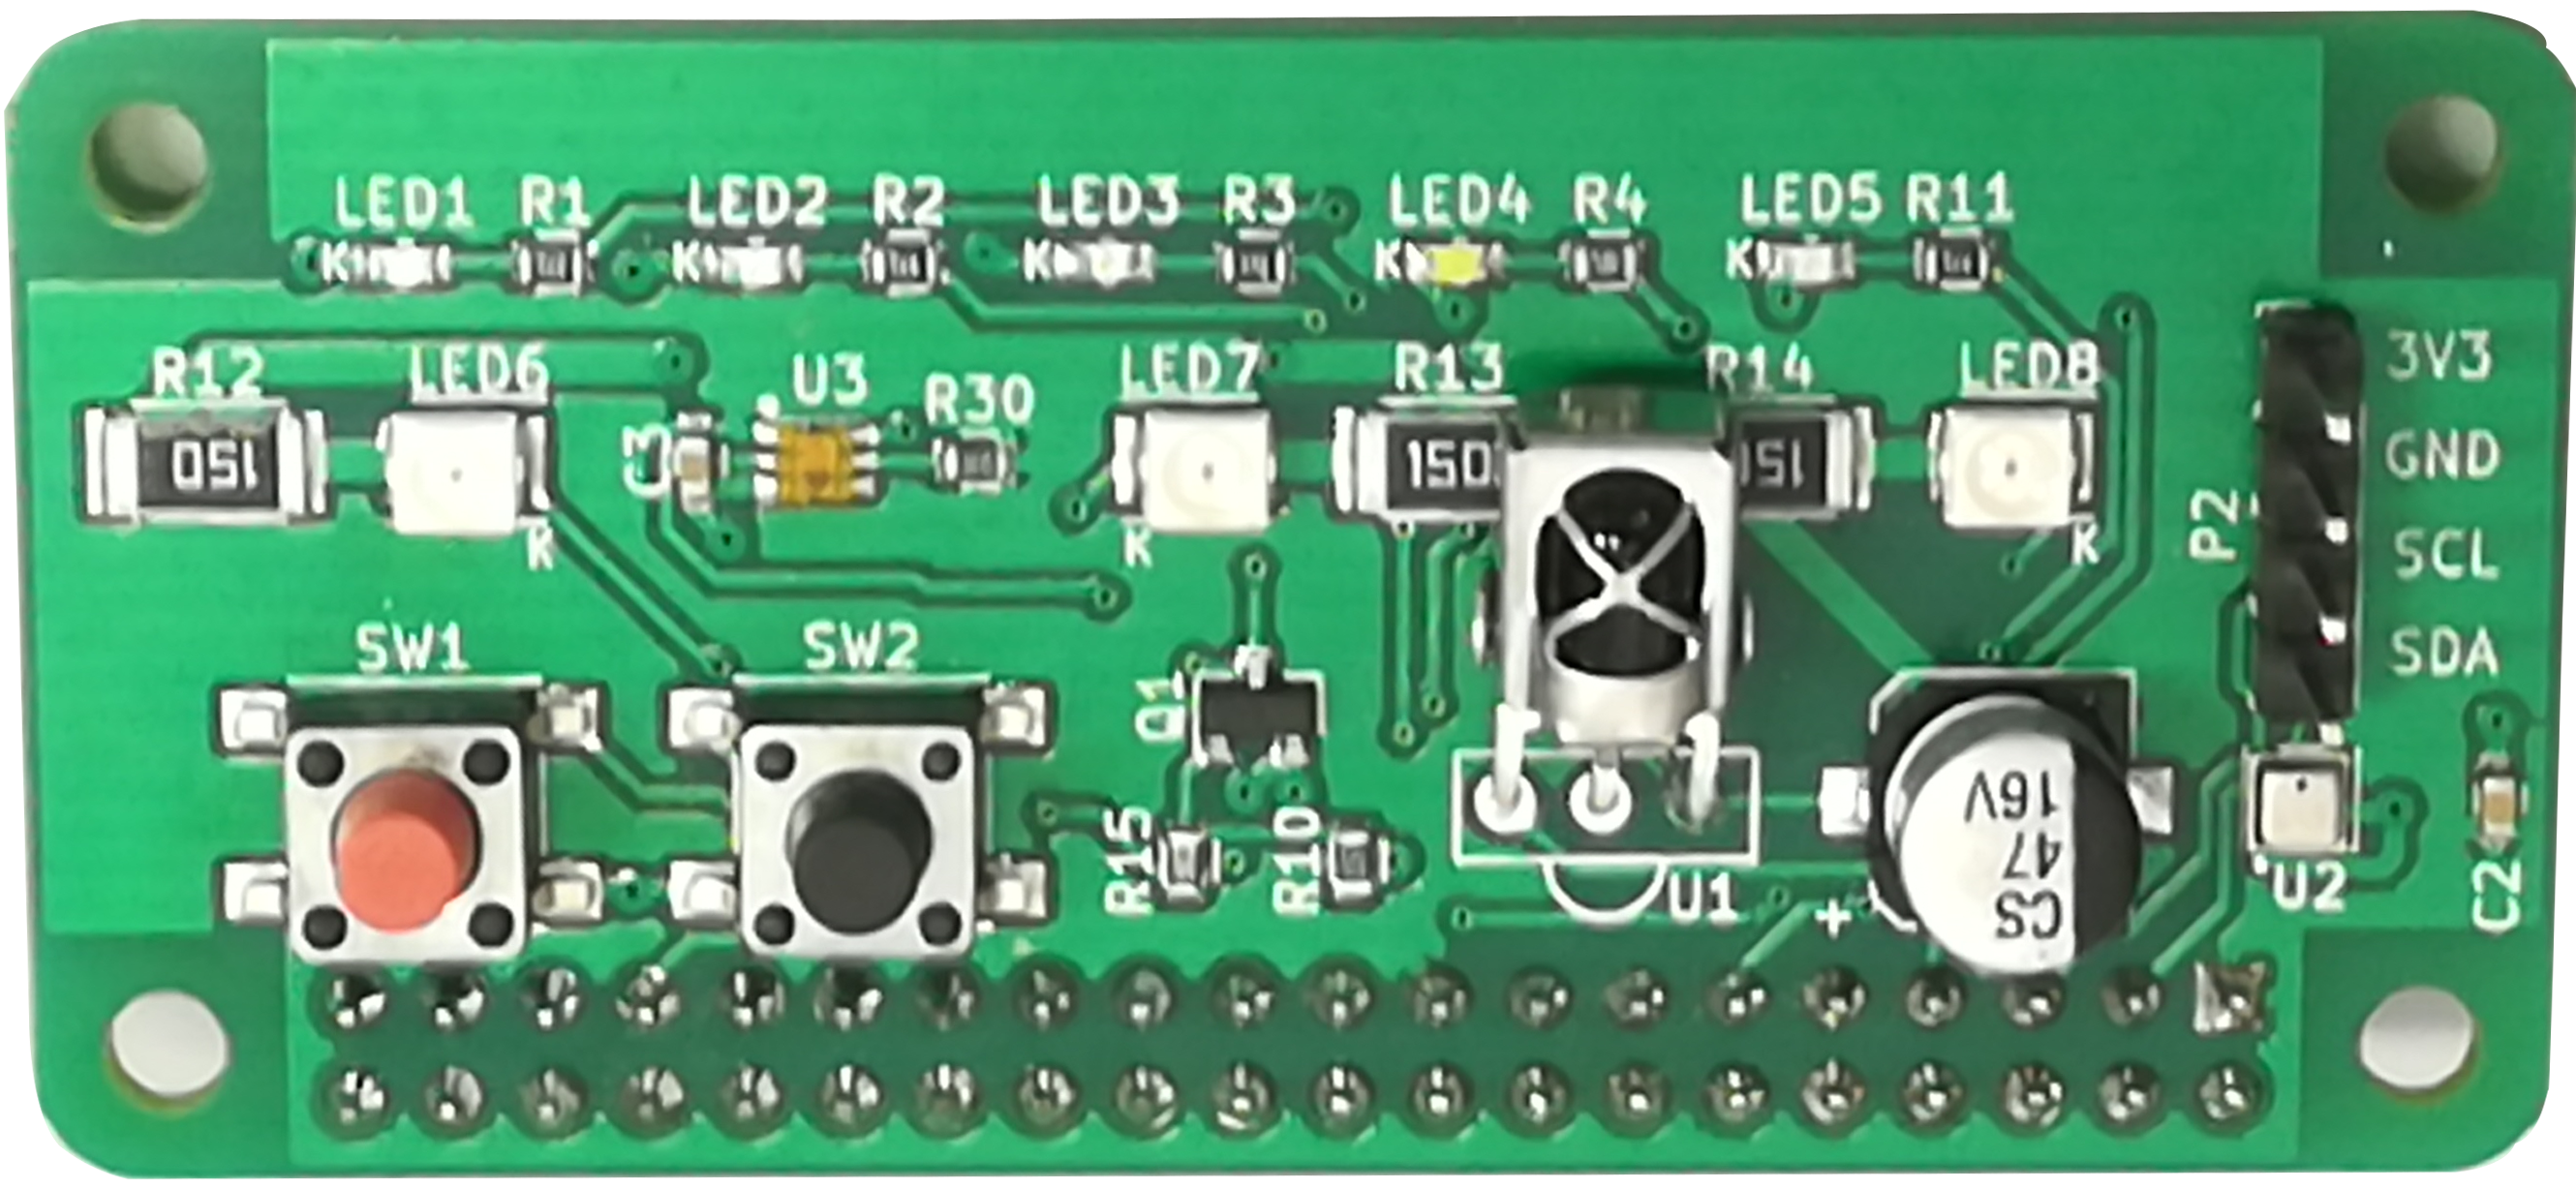
\includegraphics[width=17.006cm,height=7.849cm]{text03-img/text03-img030.png}
\end{figure}
\clearpage
センサーボードとラズベリーパイは下図のように接続されています。たとえばLED1を使つかいたいときはGPIO17というピンを使つかう必要ひつようがあります。



\begin{figure}
\centering
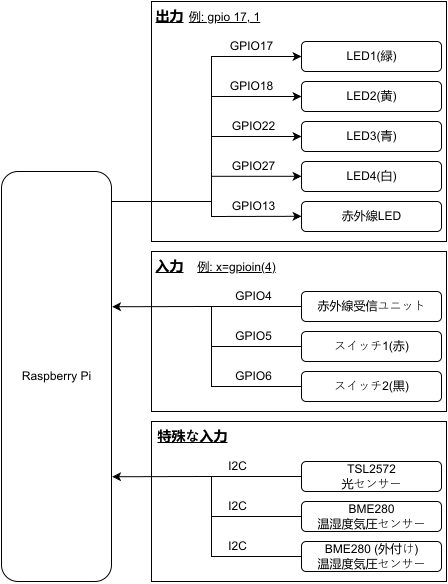
\includegraphics[width=14.982cm,height=15.942cm]{text03-img/text03-img031.png}
\end{figure}

\bigskip

\clearpage\subsection{きほんのHSPプログラム}
\subsubsection{LEDを光らせよう}
まずはセンサーボードにあるLEDを光らせてみましょう。HSPスクリプトエディタからLEDを光らせるプログラム(led.hsp)を読み込んで実行してみましょう。led.hspは、/home/pi/ome/03のディレクトリにあります。

{\ttfamily\bfseries
[Warning: Draw object ignored][Warning: Draw object ignored][Warning: Draw object ignored]\#include
{\textquotedbl}hsp3dish.as{\textquotedbl}\ \ \ \ \textcolor[rgb]{0.0,0.0,0.8}{;スクリプトの設定を読み込む}}

{\ttfamily\bfseries
\#include
{\textquotedbl}rpz-gpio.as{\textquotedbl}\ \ \ \ \textcolor[rgb]{0.0,0.0,0.8}{;スクリプトの設定を読み込む}}

[Warning: Draw object ignored]

{\ttfamily\bfseries
[Warning: Draw object ignored]\ \ redraw
0\ \ \ \ \ \ \textcolor[rgb]{0.0,0.0,0.8}{;画面更新(仮想画面に描画)}}

{\ttfamily\bfseries
\ \ font
{\textquotedbl}{\textquotedbl},30\ \ \ \ \ \ \textcolor[rgb]{0.0,0.0,0.8}{;文字のフォント、サイズを決める}}

{\ttfamily\bfseries
\ \ pos 20,20\ \ \ \ \ \ \textcolor[rgb]{0.0,0.0,0.8}{;文字の場所を決める}}

{\ttfamily\bfseries
\ \ mes
{\textquotedbl}LEDが光るよ{\textquotedbl}\ \ \ \ \textcolor[rgb]{0.0,0.0,0.8}{;文字を決める}}

{\ttfamily\bfseries
\ \ redraw
1\ \ \ \ \ \ \textcolor[rgb]{0.0,0.0,0.8}{;画面更新(実際の画面に描画)}}


\bigskip

{\ttfamily\bfseries
[Warning: Draw object ignored][Warning: Draw object ignored]*led}

{\ttfamily\bfseries
\ \ gpio 17, 1\ \ \ \ \ \ \textcolor[rgb]{0.0,0.0,0.8}{;GPIO17を点灯させる}}

{\ttfamily\bfseries
\ \ await 100\ \ \ \ \ \ \textcolor[rgb]{0.0,0.0,0.8}{;0.1秒待つ}}

{\ttfamily\bfseries
\ \ goto *led\ \ \ \ \ \ \textcolor[rgb]{0.0,0.0,0.8}{;*ledまで戻る}}


\bigskip

{\ttfamily\bfseries
\ \ gpio 17, 0}


\bigskip

下の写真のようにLEDが光りましたか?


\bigskip

[Warning: Draw object
ignored]それではプログラムを解析してみましょう。font
命令や pos 命令、
mes命令がありますね。これらがどんな命令だったかを前回の教科書を読んで復習しましょう。gpio命令も前回勉強しました。17という数字は上の接続図のGPIO17に対応していて、1という数字はONをあらわすのでしたね。

\begin{figure}
\centering
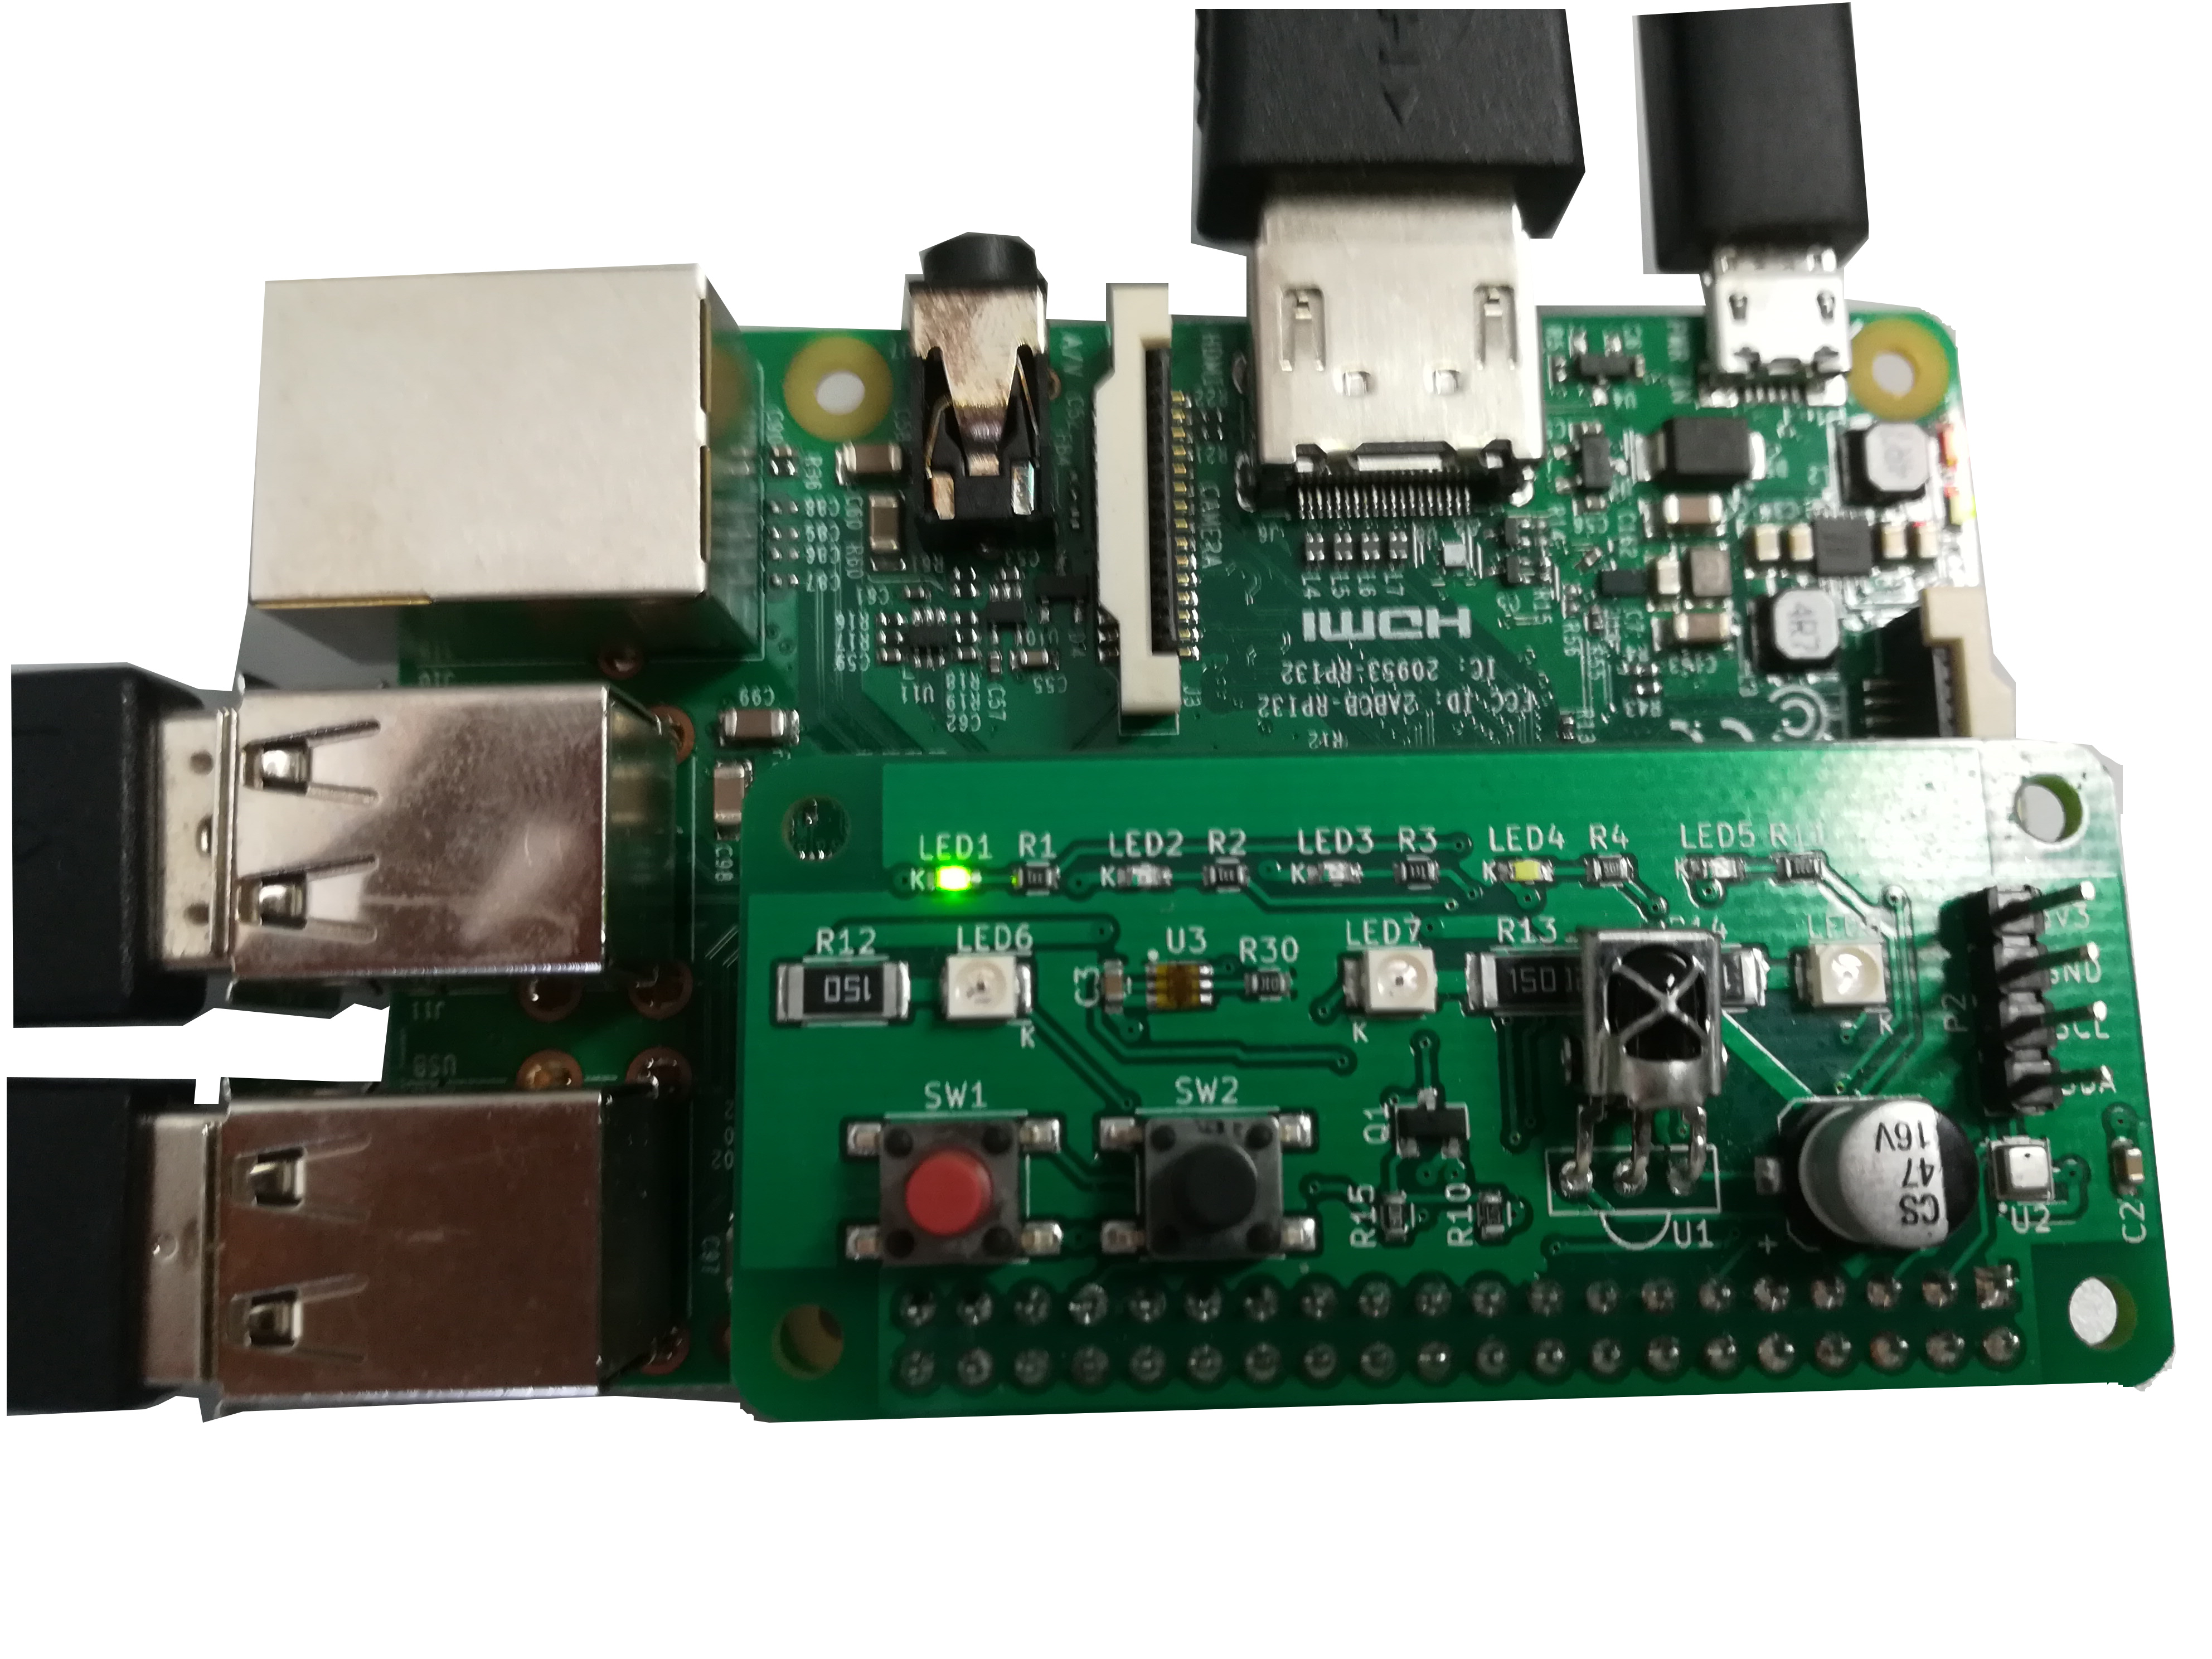
\includegraphics[width=14.369cm,height=10.776cm]{text03-img/text03-img032.jpg}
\end{figure}
{\ttfamily
問題3-16
(第2回の教科書を見ながらやりましょう)}

\begin{enumerate}
\item \begin{enumerate}
\item
LEDを光らせる命令を書きましょう(ヒント:
教科書第2回2-9
LEDが点滅するスクリプトを参考にしましょう)。


\bigskip


\bigskip

{\ttfamily\bfseries
答え.\_\_\_\_\_\_\_\_\_\_\_\_\_\_\_\_\_\_\_\_\_\_\_\_\_\_\_\_\_\_\_\_\_\_\_\_\_\_\_\_\_\_\_\_\_\_\_\_\_\_\_\_\_\_\_\_\_\_\_\_\_\_\_\_}


\bigskip
\item LEDを消す命令を書きましょう(ヒント:
教科書第2回2-9
LEDが点滅するスクリプトを参考にしましょう)。


\bigskip


\bigskip

{\ttfamily\bfseries
答え.\_\_\_\_\_\_\_\_\_\_\_\_\_\_\_\_\_\_\_\_\_\_\_\_\_\_\_\_\_\_\_\_\_\_\_\_\_\_\_\_\_\_\_\_\_\_\_\_\_\_\_\_\_\_\_\_\_\_\_\_\_\_\_\_}


\bigskip
\item
ターミナルを使ってled.hspのコピーを、321.hspという名前で作りましょう。\newline
${\square}$ $\leftarrow $
できたらチェックしましょう。
\item
他の色のLEDが光るように321.hspのプログラムを変えてみましょう。\newline
${\square}$ $\leftarrow $
できたらチェックしましょう。
\end{enumerate}
\end{enumerate}
\subsubsection{}
\clearpage\subsubsection{LEDをチカチカさせよう}
次にLEDをチカチカ(点滅)させてみましょう。HSPスクリプトエディタでLtika.hspを開いて実行してください。/home/pi/ome/03のディレクトリにあります。

{\ttfamily\bfseries
[Warning: Draw object ignored]\#include {\textquotedbl}hsp3dish.as{\textquotedbl}}

{\ttfamily\bfseries
\#include {\textquotedbl}rpz-gpio.as{\textquotedbl}}

[Warning: Draw object ignored][Warning: Draw object ignored]

{\ttfamily\bfseries
\ \ redraw 0\ \ \textcolor[rgb]{0.0,0.0,0.8}{; 画面更新
(仮想画面に描画)}}

{\ttfamily\bfseries
\ \ mes
{\textquotedbl}0.5秒毎に青色のLEDがチカチカするよ{\textquotedbl}}

{\ttfamily\bfseries
\ \ redraw 1\ \ \textcolor[rgb]{0.0,0.0,0.8}{; 画面更新
(実際の画面に描画)}}


\bigskip

{\ttfamily\bfseries
[Warning: Draw object ignored][Warning: Draw object ignored]*led}

{\ttfamily\bfseries
\ \ gpio 22,0\ \ \textcolor[rgb]{0.0,0.0,0.8}{; gpio22 を消灯}}

{\ttfamily\bfseries
\ \ wait 50\ \ \textcolor[rgb]{0.0,0.0,0.8}{; 500ミリ秒待つ}}

{\ttfamily\bfseries
\ \ gpio 22, 1\ \ \textcolor[rgb]{0.0,0.0,0.8}{; gpio22 を点灯}}

{\ttfamily\bfseries
\ \ wait 50\ \ \textcolor[rgb]{0.0,0.0,0.8}{; 500ミリ秒待つ}}

{\ttfamily\bfseries
\ \ goto *led\ \ \textcolor[rgb]{0.0,0.0,0.8}{; *led
にジャンプ(繰り返し)}}


\bigskip

プログラムを読んでみましょう。点滅させるためにはLEDのONとOFFを交互に繰り返すのでした。OFFにするgpio命令
(gpio 22, 0) と ON にするgpio命令 (gpio 22, 1)
がwait命令と交互に現れることを確認しましょう。

{\ttfamily
問題3-17
(第2回の教科書を見ながらやりましょう)}

\begin{enumerate}
\item
ターミナルを使ってLtika.hspのコピーを、322.hspという名前で作りましょう。\newline
${\square}$ $\leftarrow $
できたらチェックしましょう。
\item
ほかの色のLEDがチカチカするように322.hspのプログラムを変えてみましょう(ヒント:
教科書第2回2-9
LEDが点滅するスクリプトを参考にしましょう)。\newline
${\square}$ $\leftarrow $
できたらチェックしましょう。
\item
チカチカする速さが速くなるように、322.hspのプログラムを変えてみましょう(ヒント:
2-9
LEDが点滅するスクリプトを参考にしましょう)。\newline
${\square}$ $\leftarrow $
できたらチェックしましょう。
\item
チカチカする速さが遅くなるように、322.hspのプログラムを変えてみましょう。\newline
${\square}$ $\leftarrow $
できたらチェックしましょう。
\end{enumerate}
\begin{enumerate}
\item[] 
\bigskip
\end{enumerate}
\clearpage\subsubsection{温度、湿度(しつど)、気圧、明るさを調べてみよう}
次はセンサーボードに繋がっているBME280(温湿度気圧センサー)と、TSL2572(照度センサー)を使ってみましょう。HSPスクリプトエディタで/home/pi/ome/03/sensors.hspを読み込み実行してください。

{\ttfamily\bfseries
[Warning: Draw object ignored]\#include {\textquotedbl}hsp3dish.as{\textquotedbl}}

{\ttfamily\bfseries
\#include {\textquotedbl}rpz-gpio.as{\textquotedbl}}

[Warning: Draw object ignored]

[Warning: Draw object ignored]

{\ttfamily\bfseries
init\_bme\ \ \ \ \ \ \ \ \textcolor[rgb]{0.0,0.0,0.8}{; 温湿度気圧センサ bme280
を初期化する}}

{\ttfamily\bfseries
if stat \{\ \ \ \ \ \ \ \ \textcolor[rgb]{0.0,0.0,0.8}{;
初期化成功チェック}}

{\ttfamily\bfseries
\ \ redraw \ 0}

{\ttfamily\bfseries
\ \ mes {\textquotedbl}failed to init bme: {\textquotedbl} + stat}

{\ttfamily\bfseries
\ \ redraw 1}

{\ttfamily\bfseries
\ \ stop}

{\ttfamily\bfseries
\}}


\bigskip

{\ttfamily\bfseries
geti2c\_lux\_init\ \ \ \ \ \ \textcolor[rgb]{0.0,0.0,0.8}{; 照度センサ
tsl2572を初期化する}}


\bigskip

{\ttfamily\bfseries
*main}

{\ttfamily\bfseries
\ \ redraw 0\ \ \ \ \ \ \ \ \textcolor[rgb]{0.0,0.0,0.8}{; 仮想画面に描画}}

{\ttfamily\bfseries
\ \ pos 60, 60\ \ \ \ \ \ \ \ \textcolor[rgb]{0.0,0.0,0.8}{; 表示位置を設定}}

{\ttfamily\bfseries
[Warning: Draw object ignored]\ \ }

{\ttfamily\bfseries
[Warning: Draw object
ignored]\textcolor[rgb]{0.0,0.0,0.8}{\ \ }\textcolor{black}{get\_temp\ \ \ \ \ \ }\textcolor[rgb]{0.0,0.0,0.8}{;
rpz\_tempに温度取得}}

{\ttfamily\bfseries
\textcolor[rgb]{0.0,0.0,0.8}{\ \ }\textcolor{black}{temp = rpz\_temp}}

{\ttfamily\bfseries
\textcolor{black}{\ \ get\_humidity}\textcolor[rgb]{0.0,0.0,0.8}{\ \ \ \ ; rpz\_humに湿度取得}}

{\ttfamily\bfseries
\textcolor[rgb]{0.0,0.0,0.8}{\ \ }\textcolor{black}{hum = rpz\_hum}}

{\ttfamily\bfseries
\textcolor{black}{\ \ get\_pressure}\textcolor[rgb]{0.0,0.0,0.8}{\ \ \ \ ;
rpz\_pressに気圧取得}}

{\ttfamily\bfseries
\textcolor[rgb]{0.0,0.0,0.8}{\ \ }\textcolor{black}{press = rpz\_press}}

{\ttfamily\bfseries
\textcolor[rgb]{0.0,0.0,0.8}{\ \ }\textcolor{black}{geti2c\_lux\_als\ \ \ \ }\textcolor[rgb]{0.0,0.0,0.8}{;
rpz\_luxに照度取得}}

{\ttfamily\bfseries
\textcolor[rgb]{0.0,0.0,0.8}{\ \ }\textcolor{black}{lux = rpz\_lux}}

[Warning: Draw object ignored]

{\ttfamily\bfseries
\ \ ; 取得したデータの表示}

{\ttfamily\bfseries
[Warning: Draw object ignored]\ \ mes {\textquotedbl}温度: {\textquotedbl} + temp + {\textquotedbl}
[{\textcelsius}]{\textquotedbl}}

{\ttfamily\bfseries
\ \ mes {\textquotedbl}湿度: {\textquotedbl} + hum \ + {\textquotedbl} [\%]{\textquotedbl}}

{\ttfamily\bfseries
\ \ mes {\textquotedbl}気圧: {\textquotedbl} + press+ {\textquotedbl} [hPa]{\textquotedbl}}

{\ttfamily\bfseries
\ \ mes {\textquotedbl}照度: {\textquotedbl} + lux \ + {\textquotedbl} [lx]{\textquotedbl}}


\bigskip

{\ttfamily\bfseries
\ \ redraw 1\ \ \ \ \ \ \ \ \textcolor[rgb]{0.0,0.0,0.8}{; 実際の画面に描画}}

{\ttfamily\bfseries
\ \ wait 100}

{\ttfamily\bfseries
\ \ goto *main\ \ \ \ \ \ \ \ \textcolor[rgb]{0.0,0.0,0.8}{; 繰り返し}}


\bigskip

まずはBME280に関する行について説明します。

{\ttfamily\bfseries
init\_bme}

という命令でBME280を初期化しています。実際にはキャリブレーション(補正)のパラメータ取得をしたり、動作モードを決定したりしています。気になる方はデータシート(英語)を読んでみましょう。

この命令の値が変数
statに代入されています。初期化に失敗するとsuccessに0以外の値が入るので、次のif文で確認しています。

init\_bme によって、get\_temp, get\_humidity, get\_pressure
が使えるようになりました。

{\ttfamily\bfseries\color{black}
get\_temp\ \ \ \ \ \ ; rpz\_tempに温度取得}

{\ttfamily\bfseries\color{black}
get\_humidity\ \ \ \ ; rpz\_humに湿度取得}

{\ttfamily\bfseries\color{black}
get\_pressure\ \ \ \ ; rpz\_pressに気圧取得}


\bigskip

のようにすることによって、rpz\_tempに気温
(temperature),
rpz\_humに湿度(humidity),rpz\_pressに気圧(pressure)が入ります。

次はTSL2572に関係する行を説明します。

{\ttfamily\bfseries
init\_lux}

によってTSL2572が初期化されます。BME280のときと違って返り値を取らず、エラーチェックをする必要が無いことに気をつけましょう。実際には感度の設定等が行われます。詳しく知りたい方はデータシート(英語)を読んでみましょう。

初期化によって、geti2c\_lux\_alsが使えるようになりました。


{\ttfamily\bfseries\color{black}
geti2c\_lux\_als\ \ \ \ ; rpz\_luxに照度取得}

とすることで、rpz\_luxに照度が入ります。

これらで得られた値を変数temp, hum, press,
luxにいれていきます。

{\ttfamily\bfseries\color{black}
temp = rpz\_temp}

{\ttfamily\bfseries\color{black}
hum = rpz\_hum}

{\ttfamily\bfseries\color{black}
press = rpz\_press}

{\ttfamily\bfseries\color{black}
lux = rpz\_lux}


\bigskip

そしてこれらの変数temp, hum, press, lux
をmes命令を使って画面に表示しています。


\bigskip


\bigskip

\clearpage{\ttfamily
問題3-18}

\begin{enumerate}
\item 温度を調べる命令を書きましょう

\begin{enumerate}
\item[] 
\bigskip


\bigskip

{\ttfamily\bfseries
答え.\_\_\_\_\_\_\_\_\_\_\_\_\_\_\_\_\_\_\_\_\_\_\_\_\_\_\_\_\_\_\_\_\_\_\_\_\_\_\_\_\_\_\_\_\_\_\_\_\_\_\_\_\_\_\_\_\_\_\_\_\_\_\_\_}


\bigskip
\end{enumerate}
\item
湿度(しつど)を調べる命令を書きましょう

\begin{enumerate}
\item[] 
\bigskip

{\ttfamily\bfseries
答え.\_\_\_\_\_\_\_\_\_\_\_\_\_\_\_\_\_\_\_\_\_\_\_\_\_\_\_\_\_\_\_\_\_\_\_\_\_\_\_\_\_\_\_\_\_\_\_\_\_\_\_\_\_\_\_\_\_\_\_\_\_\_\_\_}
\end{enumerate}
\item 気圧を調べる命令を書きましょう

\begin{enumerate}
\item[] 
\bigskip


\bigskip

{\ttfamily\bfseries
答え.\_\_\_\_\_\_\_\_\_\_\_\_\_\_\_\_\_\_\_\_\_\_\_\_\_\_\_\_\_\_\_\_\_\_\_\_\_\_\_\_\_\_\_\_\_\_\_\_\_\_\_\_\_\_\_\_\_\_\_\_\_\_\_\_}
\end{enumerate}
\item
sensors.hspを起動します。センサーに触れて温度をあげてみましょう。\newline
${\square}$ $\leftarrow $
できたらチェックしましょう。
\item sensors.hsp
を起動します。センサーに息をふきかけて湿度をあげてみましょう。

${\square}$ $\leftarrow $
できたらチェックしましょう。
\item
sensors.hspを起動します。センサーを手でかくして暗くしてみましょう。\newline
${\square}$ $\leftarrow $
できたらチェックしましょう。
\end{enumerate}
\subsection{}
\clearpage\subsection{センサーを組み合わせたHSPプログラム}
\subsubsection{ボタンを使ってLEDをつけてみよう}
赤いボタンを押している間LEDが光るHSPプログラムを考えてみましょう。HSPスクリプトエディタで/home/pi/ome/03/button\_led.hspを読み込み実行してください。センサーボードのボタンのどちらかを押すとLEDが1つ点灯します。

{\ttfamily\bfseries
[Warning: Draw object ignored][Warning: Draw object ignored][Warning: Draw object ignored][Warning: Draw object
ignored][Warning: Draw object ignored]\#include {\textquotedbl}hsp3dish.as{\textquotedbl}\newline
\#include {\textquotedbl}rpz-gpio.as{\textquotedbl}\newline
\newline
 \ \ redraw 0\newline
 \ \ font {\textquotedbl}{\textquotedbl},30\newline
 \ \ pos 20,20\newline
 \ \ mes
{\textquotedbl}ボタンを押している間LEDが光るよ{\textquotedbl}\newline
 \ \ redraw 1\newline
\newline
*led\newline
 \ \ btn1 = gpioin(5)\ \ ;ボタンの状態を調べる\newline
 \ \ if btn1==0 : gpio 18, 1 : else : gpio 18, 0 \newline
\ \ ;$\uparrow
もしボタンが押されていたら、$LEDを光らせる。\newline
\ \ ;$\uparrow それ以外のときは$LEDを消す。\newline
 \ \ await 10\ \ ;0.01秒待つ\newline
 \ \ goto *led\ \ ;*ledに戻る}

%\newline
ここで出てくる新しい命令は\texttt{\textbf{gpioin}}命令です。\texttt{\textbf{gpioin()}}は\texttt{\textbf{()}}の中にボタンの番号(赤いボタンはGPIO5なので5、黒いボタンはGPIO6なので6)を書きます、

\texttt{\textbf{gpioin(5)}}で赤いボタンの状態(押されているか、押されていないか)を調べることができます。

\texttt{\textbf{btn1 =
gpioin(5)}}で、赤いボタンの状態を\texttt{\textbf{btn1}}という変数に代入しています。赤いボタンは押されている間、変数の数字が0、押されていない間は1になります。

赤いボタンが押されている間、LEDをつけたい。そこで、もし赤いボタンが押されていたら(変数の数字が0のとき)LEDを光らせる、それ以外のときは消すという命令を書きます。もし〜は\texttt{\textbf{if}}命令を書きます。\newline
\texttt{\textbf{if btn1==0 }}で\texttt{\textbf{btn1
}}変数の数字が0のとき(赤いボタンが押されているとき)は
:
の次に書かれている命令を実行します。\newline
\texttt{\textbf{: gpio 18, 1}}でGPIO18のLEDを光らせます。\newline
\texttt{\textbf{: else : gpio 18,
0}}では、else(それ以外)のとき、GPIO18のLEDを消しています。


\bigskip

\clearpage{\ttfamily
問題3-19}

\begin{enumerate}
\item
ボタンが押されているか調べる命令を書きましょう。

\begin{enumerate}
\item[] 
\bigskip
\end{enumerate}
答え.\_\_\_\_\_\_\_\_\_\_\_\_\_\_\_\_\_\_\_\_\_\_\_\_\_\_\_\_\_\_\_\_\_\_\_\_\_\_\_\_\_\_\_\_\_\_\_\_\_\_\_\_\_\_\_\_\_\_\_\_\_\_\_\_
\item
ターミナルを使ってbutton\_led.hspのコピーを、331.hspという名前で作りましょう。\newline
${\square}$ $\leftarrow $
できたらチェックしましょう。
\item
黒いボタン(GPIO6)を使ってLEDを光らせるように、331.hspのプログラムを変えてみましょう。\newline
${\square}$ $\leftarrow $
できたらチェックしましょう。
\item
赤いボタン(GPIO5)でLED1(GPIO17)、黒いボタン(GPIO6)でLED3(GPIO22)が光るように、331.hspのプログラムを変えてみましょう。\newline
${\square}$ $\leftarrow $ できたらチェックしましょう
\end{enumerate}
\clearpage\subsubsection{ボタンを使ってLEDをつけてみよう(2)}
HSPスクリプトエディタで/home/pi/ome/03/button\_led2.hspを読み込み実行してください。前のプログラムではボタンを押している間LEDがつきましたが、今度はボタンを押すたびにLEDのON/OFFが変わります。

{\ttfamily\bfseries
[Warning: Draw object ignored][Warning: Draw object ignored][Warning: Draw object ignored][Warning: Draw object
ignored][Warning: Draw object ignored]\#include {\textquotedbl}hsp3dish.as{\textquotedbl}\newline
\#include {\textquotedbl}rpz-gpio.as{\textquotedbl}\newline
\newline
 redraw 0\newline
 font {\textquotedbl}{\textquotedbl},30\newline
 pos 20,20\newline
 mes
{\textquotedbl}赤いボタンを押して、LEDをつけたり消したりできるよ{\textquotedbl}\newline
 redraw 1\newline
\newline
 ima\_btn =
1\ \ \ \ \textcolor[rgb]{0.2,0.2,1.0}{;今ボタンを押しているかどうかの変数}\newline
 mae\_btn =
1\ \ \ \ \textcolor[rgb]{0.2,0.2,1.0}{;前回はボタンを押しているかどうかの変数}\newline
 led =
1\ \ \ \ \ \ \textcolor[rgb]{0.2,0.2,1.0}{;LEDを光らせるかどうか決める変数}\newline
\newline
*hata\newline
 \ ima\_btn = gpioin(5)\newline
 \ if ima\_btn =
0\{\ \ \ \ \textcolor[rgb]{0.2,0.2,1.0}{;今押されていないとき
}\newline
 \ \ \ if mae\_btn =
1\{\ \ \textcolor[rgb]{0.2,0.2,1.0}{;前は押されていなかったとき}}

{\ttfamily\bfseries
\ \ \ \ \ \ \ \ \ \ \ \ \ gpio 22,
led\ \ \ \ \textcolor[rgb]{0.2,0.2,1.0}{;GPIO22をつけるか消すかする}\newline
 \ \ \ \ \ led = 1 -
led\ \ \textcolor[rgb]{0.2,0.2,1.0}{;LEDの消灯を切り返る}\newline
 \ \ \}}

{\ttfamily\bfseries
\ \ \ \ \}\newline
 \ mae\_btn =
ima\_btn\ \ \textcolor[rgb]{0.2,0.2,1.0}{;今の状態を前回の状態とする}\newline
\newline
 \ await 10\newline
 \ goto *hata\newline
}


\bigskip


\bigskip


\bigskip



\begin{figure}
\centering
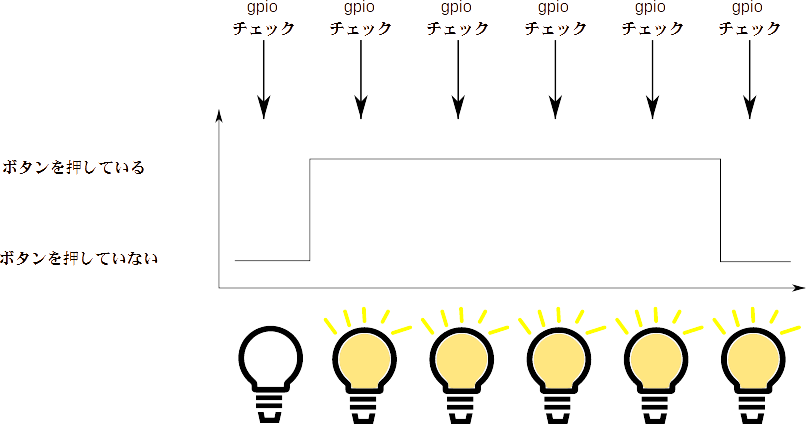
\includegraphics[width=17.006cm,height=9.495cm]{text03-img/text03-img033.png}
\end{figure}
これを実現するには
工夫が必要です。「前回はボタンが押されていたかったけど今はボタンが押されている」ときのみLEDのON/OFFを切り替える必要があります。これを「変化を検出する」といいます。

{\ttfamily
問題3-20}

\begin{enumerate}
\item
ターミナルを使ってbutton\_led2.hspのコピーを、332.hspという名前で作りましょう。\newline
${\square}$ $\leftarrow $
できたらチェックしましょう。
\item
黒いボタン(GPIO6)でLEDが点灯するように332.hspのプログラムを変えてみましょう。\newline
${\square}$ $\leftarrow $
できたらチェックしましょう。
\item
赤いボタン(GPIO5)でLED1(GPIO17)、黒いボタン(GPIO6)でLED3(GPIO22)が点灯するように332.hspのプログラムを変えてみましょう。\newline
${\square}$ $\leftarrow $
できたらチェックしましょう。
\end{enumerate}
\subsubsection{}
\subsubsection{}
\clearpage\subsubsection{ボタンを押して光るLEDを変えてみよう}
赤いボタンを押すと点くLEDが次々に変わるHSPプログラムを考えてみましょう。HSPスクリプトエディタで/home/pi/ome/03/button\_led3.hspを読み込み実行してください。

{\ttfamily\bfseries
[Warning: Draw object ignored][Warning: Draw object ignored][Warning: Draw object ignored][Warning: Draw object
ignored][Warning: Draw object ignored][Warning: Draw object ignored][Warning: Draw object ignored][Warning: Draw object
ignored][Warning: Draw object ignored][Warning: Draw object ignored][Warning: Draw object ignored]\#include
{\textquotedbl}hsp3dish.as{\textquotedbl}\newline
\#include {\textquotedbl}rpz-gpio.as{\textquotedbl}\newline
\newline
\ \ redraw 0\newline
\ \ font {\textquotedbl}{\textquotedbl},30\newline
\ \ pos 20,20\newline
\ \ mes
{\textquotedbl}赤いボタンで光るLEDを変えることができるよ{\textquotedbl}\newline
\ \ redraw 1\newline
\newline
\ \ ima\_btn = 1\newline
\ \ ledidx = 0\newline
\newline
*hata\newline
\ \ ima\_btn = gpioin(5)\newline
\ \ if ima\_btn=0 \{\newline
\ \ \ \ ledidx = (ledidx+1) {\textbackslash} 4\newline
\newline
\ \ \ \ if ledidx=1 \{\newline
\ \ \ \ \ \ gpio 17, 1\newline
\ \ \ \ \ \ gpio 18, 0\newline
\ \ \ \ \ \ gpio 22, 0\newline
\ \ \ \ \ \ gpio 27, 0\newline
\ \ \ \ \}\newline
\ \ \ \ else : if ledidx=2 \{\newline
\ \ \ \ \ \ gpio 17, 0\newline
\ \ \ \ \ \ gpio 18, 1\newline
\ \ \ \ \ \ gpio 22, 0\newline
\ \ \ \ \ \ gpio 27, 0\newline
\ \ \ \ \}\newline
\ \ \ \ else : if ledidx=3 \{\newline
\ \ \ \ \ \ gpio 17, 0\newline
\ \ \ \ \ \ gpio 18, 0\newline
\ \ \ \ \ \ gpio 22, 1\newline
\ \ \ \ \ \ gpio 27, 0\newline
\ \ \ \ \}\newline
\ \ \ \ else : if ledidx=0 \{\newline
\ \ \ \ \ \ gpio 17, 0\newline
\ \ \ \ \ \ gpio 18, 0\newline
\ \ \ \ \ \ gpio 22, 0\newline
\ \ \ \ \ \ gpio 27, 1\newline
\ \ \ \ \}\newline
\ \ \}\newline
\newline
\ \ await 10\newline
\ \ goto *hata\newline
}


\bigskip

\clearpage
\texttt{\textbf{ledidx = (ledidx+1) {\textbackslash}
4}}によって何回\texttt{\textbf{*hata}}まで戻っているか数えています。LEDは4つあるので、4回動けば一周できます。一周したらまた1に戻りたいので、割り算を使っています。今回は小数や余りは気にしなくてもいいので、\texttt{\textbf{ledidx}}は0〜4のどれかの数字になります。\newline
\newline
if 条件文1 \{実行文1\} else : if 条件文2\{実行文2\}\newline
これは条件文1が成り立つときは実行文1を実行します。成り立たないときは、条件文2が成り立つかどうか調べます。条件文2が成り立つときは実行文2を実行します。
\newline
\newline
けれど、このままだとボタンを押すたびにLEDが右どなりに動いているようには見えないですね?それはコンピュータが計算するのが早すぎるせいです。ボタンを一回押したら、ひとつ右どなりに動くようにするにはどうしたらよいでしょうか。問題3-20の「変化を検出する」を参考に問題をといてみましょう。

{\ttfamily
問題3-21}

\begin{enumerate}
\item
ターミナルを使ってbutton\_led3.hspのコピーを、333.hspという名前で作りましょう。\newline
${\square}$ $\leftarrow $
できたらチェックしましょう。
\item
赤いボタン(GPIO5)を一回押すとLEDが一個右となりに動くように、333.hspのプログラムを変えてみましょう。\newline
${\square}$ $\leftarrow $
できたらチェックしましょう。
\item
赤いボタン(GPIO5)を押すとLEDが左に移動するように、333.hspのプログラムを変えてみましょう。\newline
${\square}$ $\leftarrow $
できたらチェックしましょう。
\end{enumerate}
\subsubsection{}
\clearpage\subsubsection[チャレンジ問題明るさによってLEDをつけたり、消したりしてみよう]{チャレンジ問題\newline
明るさによってLEDをつけたり、消したりしてみよう}
これはチャレンジ問題です。レベルアップしたい人は挑戦してみてください。\newline
暗い時に全てのLEDが光るプログラムを書きましょう。3.2.3で明るさを調べる照度センサーを使いました。明るさを調べる命令(教科書27ページから)を思い出し、これまでのプログラムを参考にして、新しいプログラムを書いてみましょう。

\begin{enumerate}
\item
HSPスクリプトエディタで/home/pi/ome/03/に、light.hspという新しいファイルを作りましょう。
\item {\color{blue}
プログラムの設定をきめます。}

\begin{enumerate}
\item
\#includeを使って''rpz-gpio.as''と{}''hsp3dish.as''を読み込みましょう。
\item
ts12572に使うI2Cチャンネルを1に設定しましょう。
\end{enumerate}
\item {\color{blue}
ディスプレイに表示するものをきめます。}

\begin{enumerate}
\item
仮想画面に描画するためにredrawを書きましょう。
\item
文字をディスプレイに表示する命令を書きましょう。好きな文字を表示しましょう。
\item
実際の画面に描画するためのredraw命令を書きましょう
\end{enumerate}
\item {\color[rgb]{0.2,0.2,1.0}
明るさを調べ、暗い時にLEDをすべて光らせます}

\begin{enumerate}
\item
*mainという''はた{}''(目印)を使いましょう。
\item
明るさを調べる命令を書きましょう。
\end{enumerate}
\end{enumerate}

\bigskip

\setcounter{saveenum}{\value{enumi}}
\begin{enumerate}
\setcounter{enumi}{\value{saveenum}}
\item \setcounter{saveenum}{\value{enumii}}
\begin{enumerate}
\setcounter{enumii}{\value{saveenum}}
\item \clearpage
暗い時を考えてみましょう。暗いときは、明るさが100以下にになります。\newline
明るさが100より小さい時、LED1,LED2,LED3,LED4が光る という命令を書きましょう。条件によって実行する命令を変える場合はifを使いました。\newline
明るさが100より小さい時という条件は 明るさが入っている変数
{\textless} 100とかきます。\newline
if 明るさが100より小さい時 \{\newline
LED1を光らせる命令\newline
LED2を光らせる命令\newline
LED3を光らせる命令\newline
LED4を光らせる命令\newline
\}
\item
次に、部屋が暗くないとき(4.3の条件に当てはまらない時)を考えてみましょう。条件に当てはまらない時に、実行すり命令はelse
:\{\}の\{\}の中に書くのでした。\newline
else : \{\newline
LED1を消す命令\newline
LED2を消す命令\newline
LED3を消す命令\newline
LED4を消す命令\newline
\}
\item
プログラムの一時停止のためのwait命令を書きましょう
\item
*mainまで戻る繰り返しのgoto命令を書きましょう。
\end{enumerate}
\item
\{\}や''などの記号のつけ忘れがないか確認しましょう。
\end{enumerate}
\section{参考文献}
Indoor Corgi Elec. RPZ-IR-Sensor \url{http://indoor.lolipop.jp/IndoorCorgiElec/RPZ-IR-Sensor.php}
\end{document}
